


\documentclass[11pt]{article}
\usepackage[utf8]{inputenc}
\usepackage[english]{babel}
\usepackage[round]{natbib}
\setcitestyle{authoryear,open={(},close={)}} 


\usepackage{mathpazo, amsmath, amssymb, amsfonts, amsthm, microtype, tikz, titling, graphicx, booktabs, caption, subcaption, bm, xfrac, appendix, setspace, comment, float, nth, fnpct, makecell, multirow, tabularx, threeparttable, titling, array, lipsum, mathtools, tocloft}


%\bibliographystyle{abbrvnat}
\usepackage{enumitem}
\usepackage{graphics}
\usepackage{url}
\linespread{1.5}
\usepackage[margin=0.8in]{geometry}
\usepackage{hyperref}
\usepackage{comment}

\hypersetup{
    colorlinks,
    linkcolor={blue!80!black},
    citecolor={blue!90!black},
    urlcolor={blue!90!black}, 
   % urlbordercolor=red,
   % linkbordercolor=red,
   % citebordercolor=red,
   % runbordercolor=red,
   % citebordercolor=red,
    %filebordercolor=red
}


\usepackage{xcolor}
\usepackage{graphicx}
\usepackage{url}
\usepackage[round]{natbib}
\usepackage{amsmath,amsthm} 
\usepackage{engord}
\usepackage{float}
\usepackage{subfig}
\usepackage{pdflscape}
\usepackage{booktabs}
\usepackage{pgfplots}
\usepackage{titleps}
\usepackage{setspace}
\usepackage{dcolumn}
%\usepackage{subcaption}

%references
\usepackage{cleveref}

%%%%%%%
\usepackage{blindtext}
\usepackage{tabularx}
\usepackage{bbold}
%%%%%%%
\usepackage{multirow}
\usepackage{xr}
\usepackage{setspace}
\usepackage{sectsty}
\usepackage[labelsep=period]{caption} %% This switches %"Table 1: itle" to "Table 1. Title"
\usepackage{rotating}
\usepackage{graphics}
\usepackage{fancyhdr, ifthen}
\usepackage{blindtext}
\usepackage{pdflscape}

	
\usepackage{lineno}
%\linenumbers


\usepackage{amssymb}
\newtheorem{prediction}{Prediction}

\usepackage{appendix}
\newcommand{\Appendixautorefname}{appendix}

%%%%%%%%%%%%%%%%%%%%%%%%%%%%%%%%%%%%%%%%%

\newcommand{\footremember}[2]{%
    \footnote{#2}
    \newcounter{#1}
    \setcounter{#1}{\value{footnote}}%
}

\newcommand{\footrecall}[1]{%
    \footnotemark[\value{#1}]%
} 

% Adjust vertical space between main text and footnotes
\skip\footins=2\baselineskip plus 4pt minus 2pt

%\setlength{\footnotesep}{\baselineskip}

\usepackage{multicol}

\usepackage{threeparttable, booktabs, adjustbox}

\usepackage{subfig} % Required for subfigures

\usepackage[bottom]{footmisc} % Ensure footnotes are always at the bottom

%\flushbottom
%\raggedbottom
%\interfootnotelinepenalty=10000
\interfootnotelinepenalty=10000 % Set a high penalty




%%%%%%%%%%%%%%%%%% TITLE %%%%%%%    %%%%%%%%

\title{\centering The Political Legacy of Displacement: \\ Evidence from the Spanish Exile\footnote{\footnotesize We wish to express our sincere gratitude to Hillel Rapoport, Giovanni Peri, Victor Gay, Andreas Steinmayr, Tanya Surovtseva, 
Mario Carillo, Cédric Chambru, Ángel Herrerín, Paul Maneuvrier-Hervieu, Josepa Miquel-Florensa  and Ricardo Turati, as well as all participants of the 8th Economics and Politics Workshop, the Congrès de l'Association Française d'Histoire Economique. }}
\author{
Cristina Aranzana\footnote{University of Barcelona. Email: \href{mailto:c.aranzana@ub.edu}{c.aranzana@ub.edu}} \and
Luc Paluskiewicz\footnote{Paris School of Economics, Collège de France. Email: \href{mailto:luc.paluskiewicz@psemail.eu}{luc.paluskiewicz@psemail.eu}}
}

\date{ This version: \today \\ \href{https://www.dropbox.com/scl/fi/olo8q2405bpl3xrcra1wg/Draft_Aranzana&Paluskiewicz.pdf?rlkey=61dwvuv15u9m3tsyofifhk8m0&st=ekrs2y9v&dl=0}{[Click here for the latest update]}. }




%%%%%%%%%%%%%%%%%% TEXT %%%%%%%%%%%%%%%

\begin{document}

\maketitle  

\thispagestyle{empty}

\begin{abstract}

\noindent 

This paper studies the long-run political consequences of forced displacement when refugees are politically selected. In 1939, the collapse of the Spanish Republic triggered the sudden arrival of nearly 500,000 left-leaning refugees in France. French authorities, unprepared for the scale of the inflow, interned the displaced population in camps whose locations were determined primarily by logistical constraints. We exploit this quasi-random location of the camps to identify the causal impact of refugee exposure on local political behaviour. Municipalities hosting camps experienced a persistent decline in support for the socialist party, consistent with political backlash. Meanwhile, exposure increased support for the Communist Party and increased the number of individuals involved in the resistance, in line with the diffusion of political ideas. Taken together, the results show that the arrival of politically motivated refugees can generate political polarisation. 

\end{abstract}

\newpage

\setcounter{page}{1}
\section{Introduction}\label{sec:introduction}

As of the end of June 2025, 117.3 million people had been forced to flee their homes globally due to violence, conflict and human rights violation (UNHCR, 2025). When persecution is politically motivated, exile becomes politically selective. What are the political consequences for host communities when they receive ideologically motivated refugees? Contact between the displaced and the native population could not only reduce prejudice \citep{allport1954prejudice}, but also facilitate the diffusion of ideas between both groups. On the contrary, if the integration of the displaced population is limited, the ideas refugees bring may be perceived as a specific threat, generating political backlash. Perceptions of threat could be amplified when the displaced population is politically distant. Theoretically, the expected effect is therefore ambiguous.


To examine this question, we focus on the mass exodus from Spain to France during the final phase of the Spanish Civil War, known as La Retirada (``the retreat”). In early 1939, the collapse of Republican forces in Catalonia—who represented various left-wing groups including anarchists, communists, and other republican factions—triggered the flight of nearly half a million people. French authorities, unprepared for the scale of the inflow, treated the refugees as a security concern and responded by interning them. The locations were chosen under extreme time pressure based on logistical availability. Because no permanent facilities had been prepared in advance, the selection of camp sites was improvised. In the South, remote beaches, open plains, and abandoned barracks were selected primarily for their availability and their capacity to confine large numbers of people \citep{Coignard2012, dreyfus-armand_refugies_2016}. This process generated a geographically uneven yet plausibly exogenous distribution of camp locations.

Spanish refugees were regarded as ``undesirable foreigners” and seen as an economic burden. Therefore, propaganda and incentives were used to promote ``voluntary” repatriation to Spain or emigration to third countries. By early August, nearly half of those who had crossed the border during the episode had gone back \citep{perez_rodriguez_indeseables_2022}. Among those who remained, many were recruited into labour and military service. With the onset of World War II, their situation deteriorated further: some joined the French Resistance, while thousands were captured and deported to Nazi concentration camps. By the end of the World War II, 160,000 Republican exiles were still living in the country \citep{Coignard2012}. This allows us to study the effect of exposure to a refugee camp without the results being completely driven by subsequent changes in the demographic composition of the population or the economic structure, as most of the Spanish population eventually left the municipalities.

By leveraging this historical episode, we exploit the improvised placement of camps and estimate their effect on voting behaviour using a difference-in-differences strategy that accounts for spatial spillovers. Exposure to a refugee camp decreased the share of votes to the socialist party by 2,7 percentage points. Given that the refugees were themselves strongly aligned with left-wing and socialist ideals, this decline is consistent with a political backlash among host populations.

Yet the response was not uniform across the political spectrum. Several classic left-wing organizations—particularly labour and professional unions—were actively involved in assisting the refugees and thus maintained close contact with them. This heterogeneity is reflected in our findings. We observe a positive impact on support for the Communist Party - municipalities within 1 km away from the refugee camp increased their share of vote for the communist in 1,6 percentage points.In line with these results, municipalities that hosted refugees exhibit higher levels of mobilization against the Nazi occupation, indicating that exposure also fostered forms of political engagement aligned with the refugees’ ideological profile. Neighbouring municipalities show similar positive relationships, pointing to meaningful spillover effects beyond the immediate location of the camps.  


Our research relates to the broad literature on the political effect of immigration. Much of the existing literature emphasizes recent immigration trends and their immediate impact on public opinion and political behavior \citep{halla_immigration_2017, dustmann_refugee_2018, steinhardt_xenophobic_2018}. \citet{steinmayr_contact_2021} demonstrates that the type of contact matters: in Upper Austria, temporary refugee passage towards Germany in 2015 increased far-right voting, whereas longer-term settlement reduced it. In the French context, studies have found that larger immigrant populations tend to correlate with stronger electoral performance for the Front National at the département level \citep{edo_immigration_2019}. However, this pattern does not hold at the more localized municipal level, where the relationship appears to be reversed \citep{della2013competitive, vasilopoulos2022residential, vertier_dismantling_2023}. \citet{dazey_mosque_2024} finds that support for the Front National tends to rise in polling stations located at moderate distances from mosques, but declines beyond that range. We contribute by studying the consequences of an historical event, which allows us to explore the effect in the long-term.

Moreover, our study is also linked to the literature on migration and the transmission of political ideas \citep{spilimbergo_democracy_2009, barsbai_effect_2017, dippel_leadership_2021, calderon_racial_2023, bazzi_confederate_2023}. Previous research concentrates mostly on the effect at the origin country, with the exception of \citet{dippel_leadership_2021}, who study how the leaders of the failed German revolution of 1848–1849, expelled to the United States, positively influenced antislavery culture. We do not focus on the effects of a small political elite, as most government officials emigrated to Latin America \citep{alted2005vencidos}, but rather on a politically selected general population, which makes the analysis particularly relevant considering contemporary refugee flows. 

\section{Historical Context}\label{sec:context}



The Spanish Civil War starts in 1936 and opposes the Republican forces - composed of left-wing factions as the communists, anarchists, and socialists - and the Nationalists groups, led by General Francisco Franco and supported by fascist and conservative groups. The Nationalists won in 1939, establishing a dictatorship that lasted until 1977. By early 1939, Catalonia was one of the last Republican territories and had welcomed many internally displaced people. After the fall of Barcelona and the Nationalist offensive across Catalonia, the Republican defeat became inevitable. This collapse triggered the mass exodus of about 500,000 Spanish Republicans to France between late January and mid-February 1939. Both combatants and civilians crossed the Pyrenees in search of refuge, producing the largest sudden population movement ever recorded at the Franco-Spanish border. This influx represented a substantial demographic shock for France, representing 22\% of the country’s total foreign population according to the last pre-war census of 1939.

%Considering the last census available of 1936, the total population of France was 41967056 habitants, this represents 1,19% of the population. The shock represents 22% of the total foreign population in 1939. The total foreign population was 2198236 in 1939. The most important groups are: 721000 italians which represented 33% of the foreign population. Polish: 423000 (19percent) and Spanish 254000 (12percent). 

This sudden influx, concentrated over a few weeks, overwhelmed the French authorities who were unprepared for its scale \citep{rafaneau20081939}. Worn down by economic crisis, plagued by xenophobic sentiment, and increasingly isolationist, French authorities offers Spanish refugees a hostile reception \citep{Coignard2012}. For French authorities, still reeling from World War I, the priority was to maintain the public order and security. They were particularly worried about the spread of radical left-wing ideas, so the incoming Spaniards were treated as a security problem and were interned and dispersed all over the country \citep{rafaneau20081939}. 

Families were often separated at the border, and the civilian population was transferred to reception centres dispersed across the country. Around 170,000 of them were women, children, and elderly people \citep{perez_rodriguez_indeseables_2022}. Meanwhile, most men (particularly those of military age) were interned in improvised camps - ``concentration camps” as they were officially called - near the border in the south \citep{DreyfusArmand1999}. The legal basis for this camp system had been laid shortly before: in November 1938, the Daladier government passed a decree-law allowing the internment of “undesirable foreigners” under surveillance. The Spanish were the first to suffer the consequences of this new policy \citep{eurom_argeles-sur-mer_2014}. 

As no permanent facilities had been prepared in advance, the selection of camp sites was improvised. The very first camps were in the Pyrénées-Orientales (French Catalonia) along the Mediterranean coast: notably Argelès-sur-Mer, Saint-Cyprien, and Le Barcarès, all essentially stretches of beach beach and open fields demarcated and enclosed with barbed wire \citep{Coignard2012}. Soon, additional camps were created deeper inside France to alleviate the severe overcrowding. By the spring of 1939, a second ring of internment camps extended across the Pyrenees and southwestern France. Key camps included Gurs (in Béarn, near Pau), Le Vernet d’Ariège (in the Ariège department), Septfonds (Tarn-et-Garonne), Bram (Aude), Agde (Hérault), and Rieucros (Lozère) \citep{Coignard2012}. In the rest of the departments, the types of accommodations varied widely, whether suitable for hosting people (schools, holiday centres, sanatoriums, barracks, uninhabited houses...) or not initially appropriate (former factories, stud farms, stables, mills, village halls) \citep{DreyfusArmand1999}.

%if it was the prefect who had to give the census of places, they are elected each two years and not on the same level than the commune. so you can argue that the political tendencies did not matter that much. 

From the moment the refugees arrived, French authorities aimed to reduce the number of Spaniards on French soil. Concerned about the financial cost, they  promote ``voluntary" return through incentives and coercion. By early August, around 250,000 refugees had returned to Spain \citep{perez_rodriguez_indeseables_2022}. Moreover, around 20,000 people emigrated to other countries, with over 15,000 going to Latin America. As a result, the number of Spanish refugees and political exiles in French territory had reached approximately 180,000 individuals by December 1939 \citep{rafaneau20081939}. As World War II approached, France began to see those who remained as a valuable labour force for its war effort. In April 12, 1939, Foreign Worker Companies (Compagnies de Travailleurs Étrangers, CTE) were established to conscript refugees into labor units \citep{Coignard2012}. By the end of December, 50,000 to 60,000 Spanish refugees were working in these groups particularly along the Italian border and on Maginot Line fortifications \citep{rafaneau20081939}. In addition, the French military encouraged Spanish veterans to enlist in the armed forces. Thousands chose to join the French Foreign Legion or other military groups as a way to leave the camps \citep{perez_rodriguez_indeseables_2022}. When France fell to German forces in June 1940, Spanish refugees faced new dangers. Many men were captured and held as prisoners of war, and thousands of Spanish Republicans were subsequently deported to Nazi concentration camps—most notoriously Mauthausen, where around 7,000 died. Others managed to evade capture and join the French Resistance in significant numbers. It is estimated that up to 15,000 Spaniards participated in the French Resistance or served in the Free French forces between 1940 and 1944 \citep{academicoup}. By the end of the Second World War, it is estimated that 100000 Spanish republicans were still in the country \citep{perez_rodriguez_indeseables_2022}















\section{Data}\label{sec:data}
Information on the locations of refugee camps and centers is drawn from \citet{generalitat_de_catalunya_relacio_2020}. The information in the dataset comes from two original sources in the regional archives: \textit{Dossier on the International Conference for Aid to Spanish Refugees} (Paris, July 15–16, 1939), prepared by the Bureau d'Information (ANC1-511-T-332), and \textit{List of Cities and Towns in France with Camps or Shelters for Spanish Refugees} (ANC1-511-T-349).

%resistance data
To examine the effects on political outcomes, we draw on city-level electoral data from legislative elections compiled by \citet{piketty_histoire_2023}. We restrict the analysis to Metropolitan France and to the years 1919–1956, since 1958 marks the beginning of the Fifth Republic. In order to measure the participation into the French Resistance during the Second World War, we use public available records from the French Ministry of Armies \citep{ministry_of_the_armed_forces_memoire_2022}. Namely, we use records of official recognitions of resistance activities (\textit{Titres, homologations et services pour faits de résistance}), and recipients of resistance medals (\textit{Médaillés de la résistance}). These nominative registers provide information on age, nationality, year and place of birth at the municipality level. We locate involvement in the resistance using place of birth, considering the bad quality of the place of recruitment or death in the dataset. 

%We explore as an outcome also the effect on collaboration with the Nazi Occupation using data on the number of collaborators at the city level from \citet{cage_heroes_2023}.

We use several sources of data to check for the exogeneity of the dispersion policy. Unfortunately, no direct measure of the foreign-born population exists at the municipal level for the period. To approximate pre-existing immigrant presence, we construct a proxy based on national death records from 1970 to 2025 \citep{insee_deces_2025}. From these records, we identify French individuals with Spanish, Italian, or Portuguese surnames and recover their municipality of birth. Using this information, we reconstruct the pre-1939 shares of residents with foreign-origin surnames for each municipality. To identify which surnames are of Spanish origin, we count the frequency of surnames within the population born in Spain and use this to generate a list of common Spanish surnames. Housing availability is proxied using a measure of buildings constructed by 1939 \citep{insee1968logements} and the number of associations is drawn from the legal registry of organisations \citep{dila_journalofficiel_portal}. Finally, we include variables capturing geographic and economic structure—altitude, precipitation, and mining activity \citep{pauling2006,camino2021}. 


%To explore whether the camp locations predict the settlement of the refugees, we use the census of 1962, which is the earliest census available \citep{insee_1962}. To measure the intensity of collective actions after WWII, we rely on various archival sources that enable us to compile an inventory of all political activities carried out by Spanish refugees between 1945 and the fall of the dictatorship in Spain in 1977. We mainly gather information on the two main Spanish unions at the time of the Civil War, the \textit{Unión General de Trabajadores} (General Union of Workers, UGT) and the \textit{Confederación Nacional del Trabajo} (National Confederation of Labor, CNT). For both organizations, we are able to identify local branches of these unions and track their years of activity over time. 

%For the UGT, we use the documentations from the \citep{FFLC_ugt}. More precisely, we use an inventory of all UGT activity outside of Spain during the time of the dictatorship. This inventory gives a list of all municipalities that have had a local section of the UGT, with its date of creation. For the CNT, we use data collected from 2 sources. The first one is the \citep{FAL_cnt}, from which we use the report of general assembly of the movement in exile in 1948. This document enables us to have a precise list of all municipalities in France were Spanish refugees settled down and wished to organize politically into one new local section of the CNT after WWII. Unfortunately, since this does not allow us to track the activity of sections through time, we complete this first source with documentations from the the archives of the \citep{CDHS_cnt}. From this source, we use a large set of documents, especially meeting reports from local sections in exile. This allows us to determine the years of activity of all local sections. Using the same reports, we are able to infer the number of persons affiliated to each local sections using the subscription of news members.



\section{Descriptive statistics}\label{sec:descriptives}

%Faced with the possibility of having to receive a significant number of Spaniards, the Minister of the Interior first requested a census of all public or private premises available in the departments, particularly those that could be used to house refugees (Note d'information du Ministère de l'Intérieur envoyée aux préfets le 26 janvier 1939). Secondly, he called for contact to be made with private initiatives—especially the Red Cross, but also other philanthropic organizations—with the aim of involving them in humanitarian efforts. Lastly, a cost estimate was requested for the construction of barracks in locations that met all necessary conditions for hygiene, sanitation, and supply \citep{perez_rodriguez_indeseables_2022}. 

According to the data, up to the month of July 1939, there were 990 camps in France, hospitals or shelter centres with Spanish exiles in France. Regarding the refugees, 167,932 were combatants, most of whom were spread over 10 concentration camps, 3 hospitals and 2 refugee centres. The rest, a little over 150,000 people, civilians of both sexes and of various ages, were spread over the numerous refugee centres that extended throughout French territory. Most of these centres were managed by the host country itself, while 73 were subsidised by other countries \citep{generalitat_de_catalunya_relacio_2020}. \Cref{fig:map_camps} displays the geographical distribution of internment camps across France in 1939. Camps were not concentrated in a single region but spread widely, with notable clusters in the southern departments near the Spanish border as well as in central and western France. The size of the circles reflects camp capacity, highlighting a particularly dense presence in the Pyrenean area where the first wave of refugees entered. This distribution suggests that exposure to refugees varied considerably across municipalities. 

\begin{figure}[h!]
  \centering
  \caption{Location of the refugee camps}
  \label{fig:map_camps}
  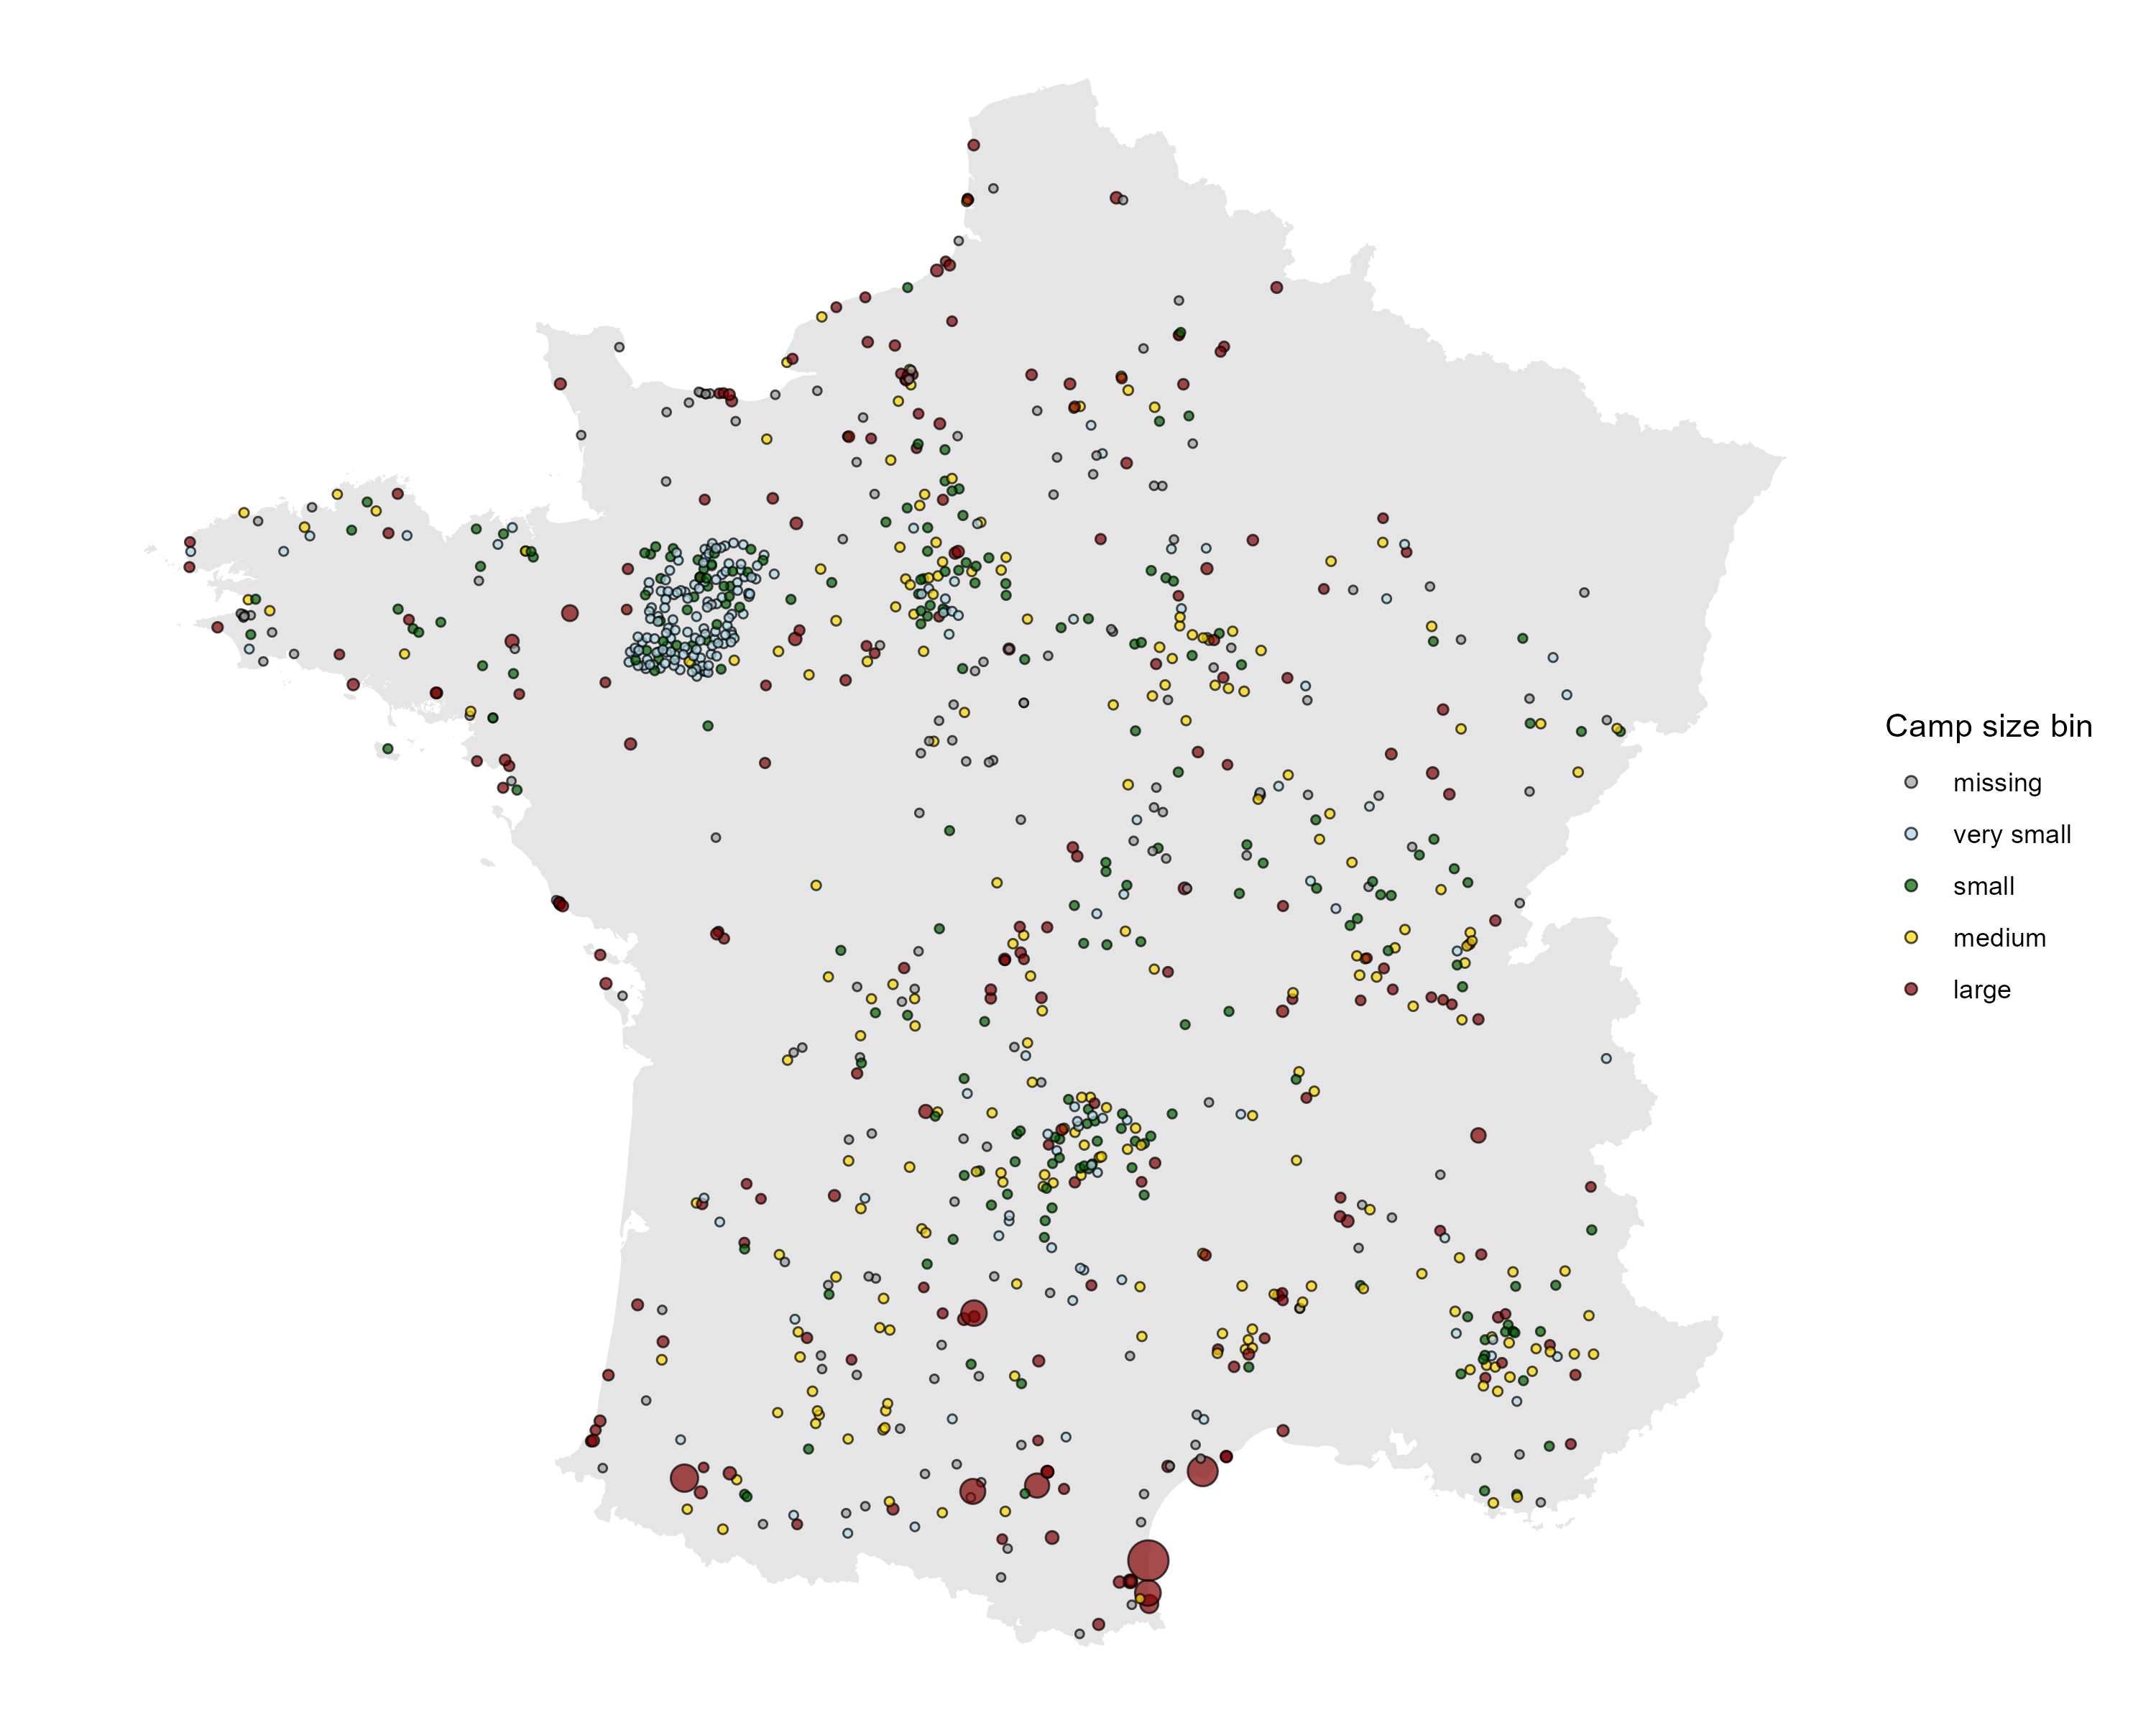
\includegraphics[width=0.8\linewidth]{figures/descriptives/maps/map7.png}
\end{figure}



\begin{figure}[h!]
    \caption{Locations of the Refugees Camps}
    \centering
    \begin{minipage}{0.49\textwidth}
        \centering
        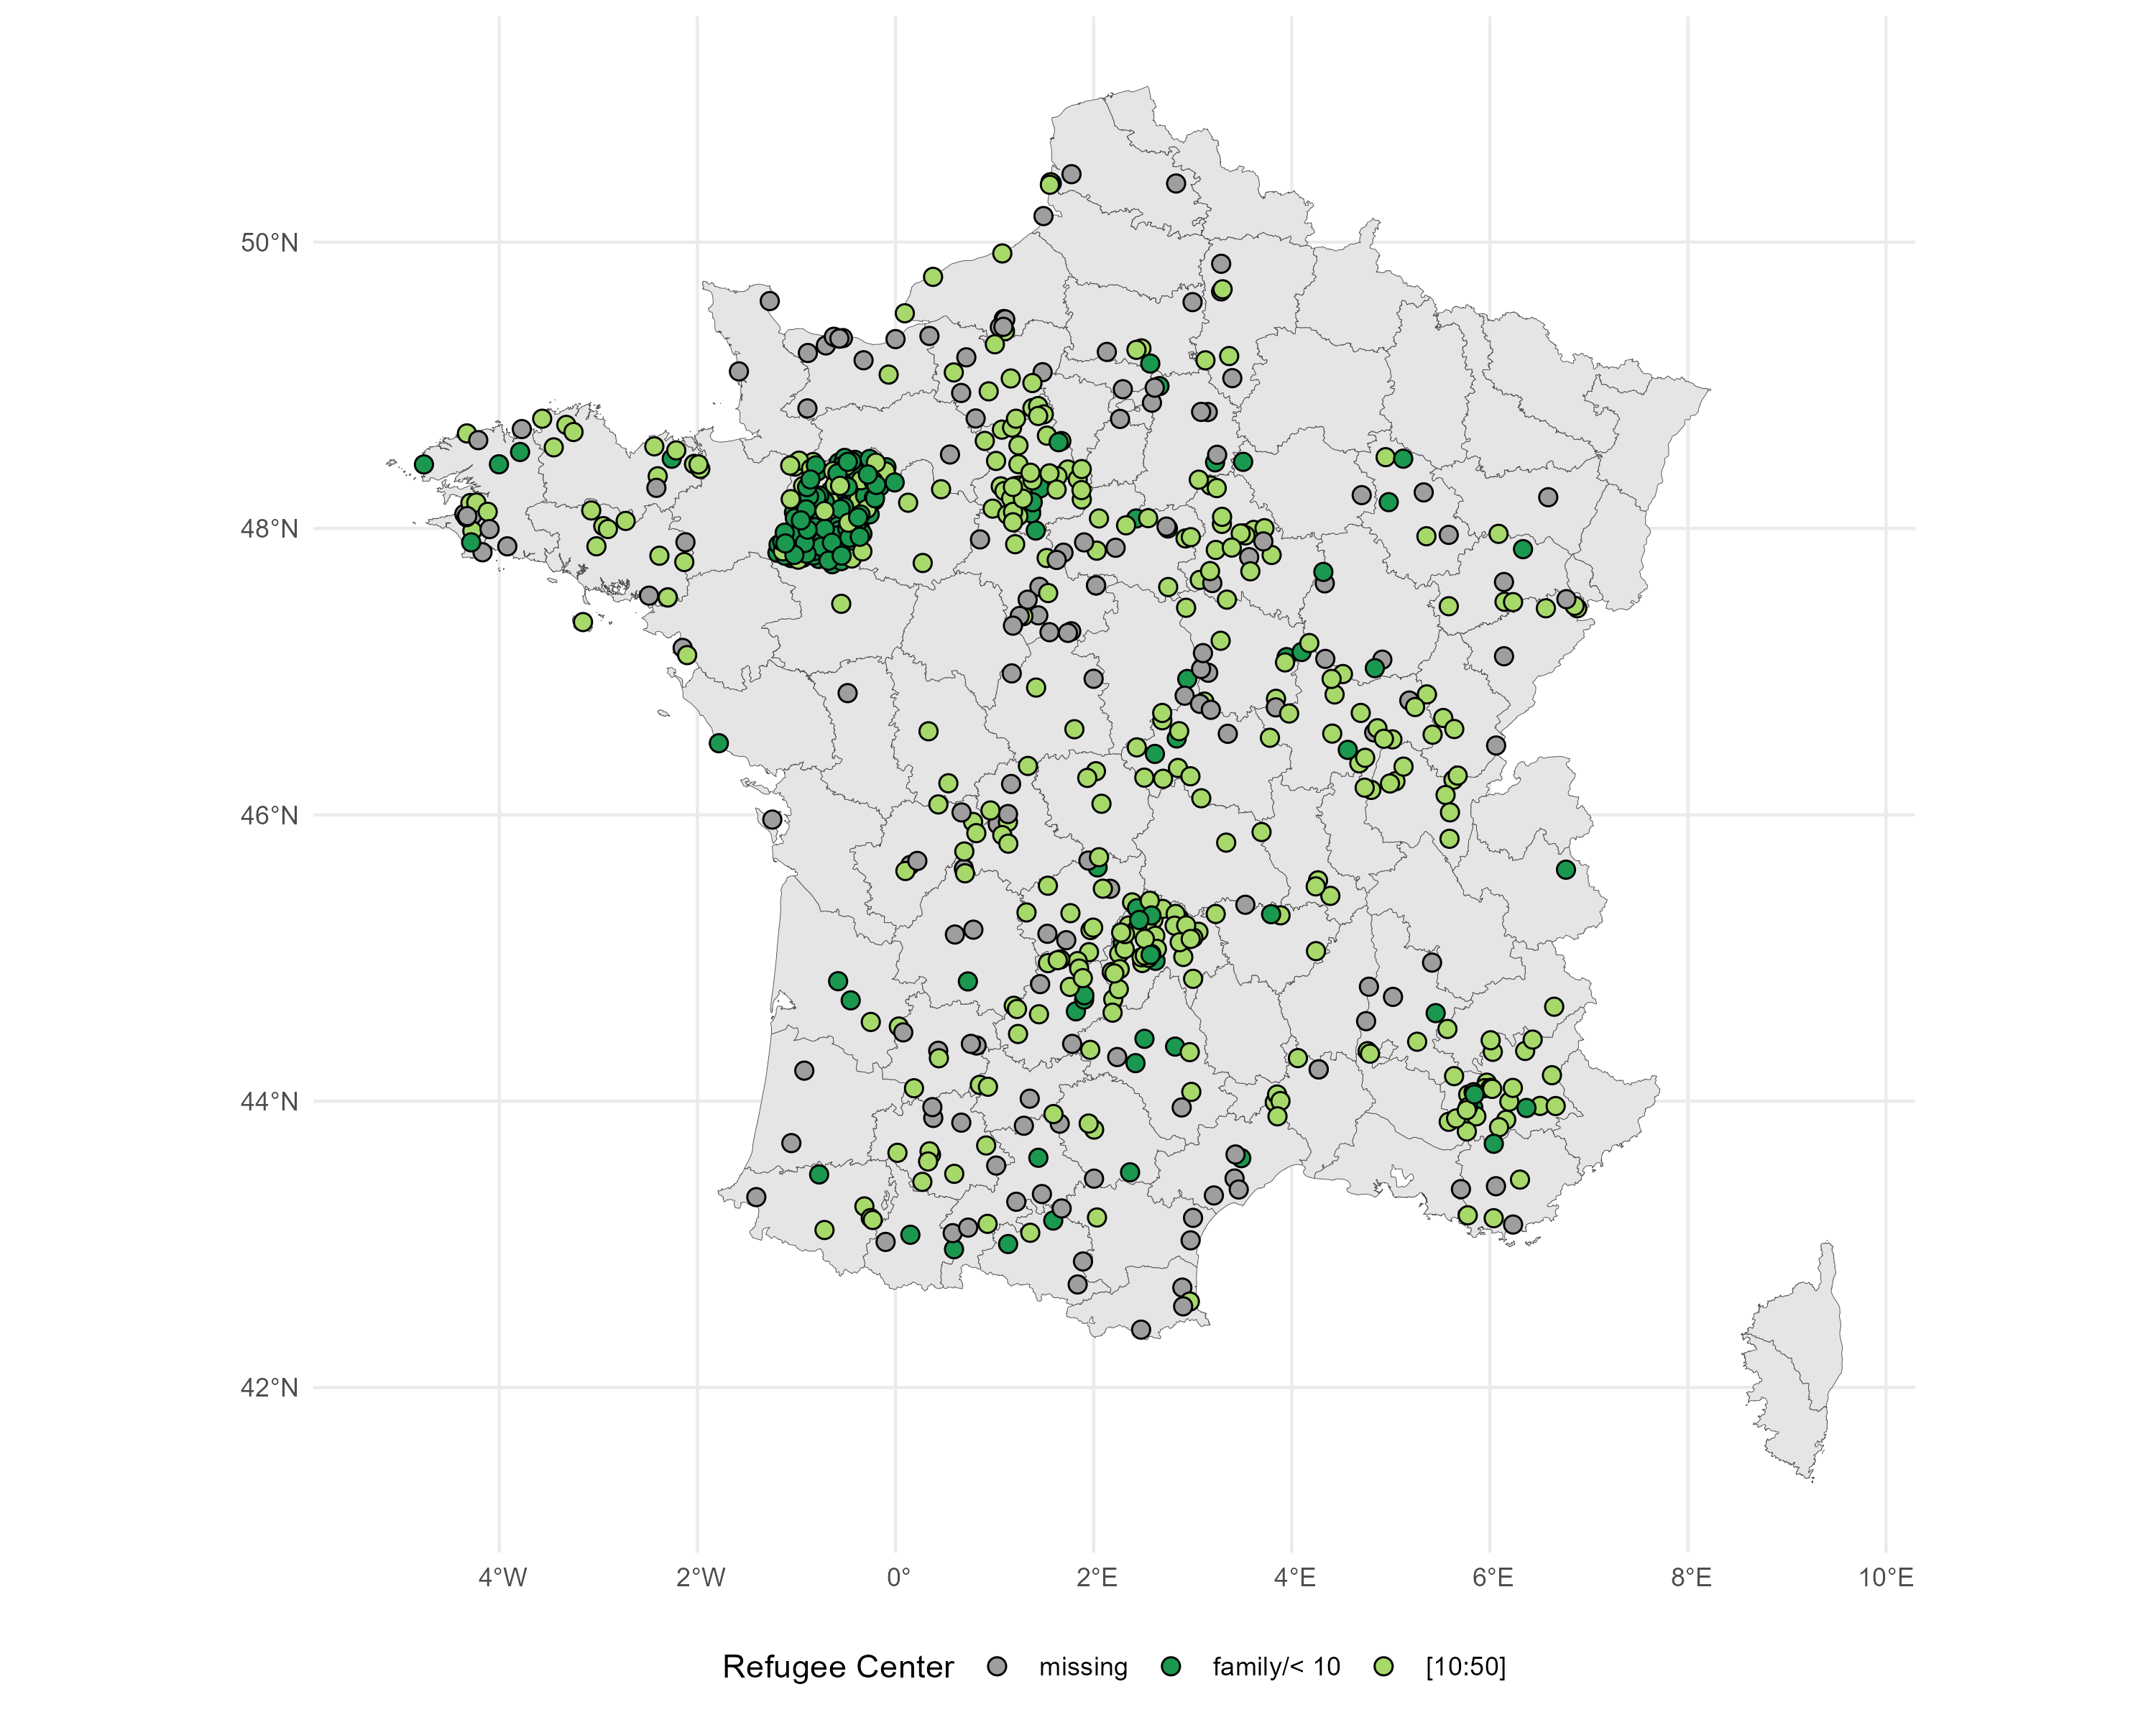
\includegraphics[width=\linewidth]{figures/descriptives/maps/map7.1.png}
        \subcaption{Missing, very small and small camps }
    \end{minipage}
    \hfill
    \begin{minipage}{0.49 \textwidth}
        \centering
        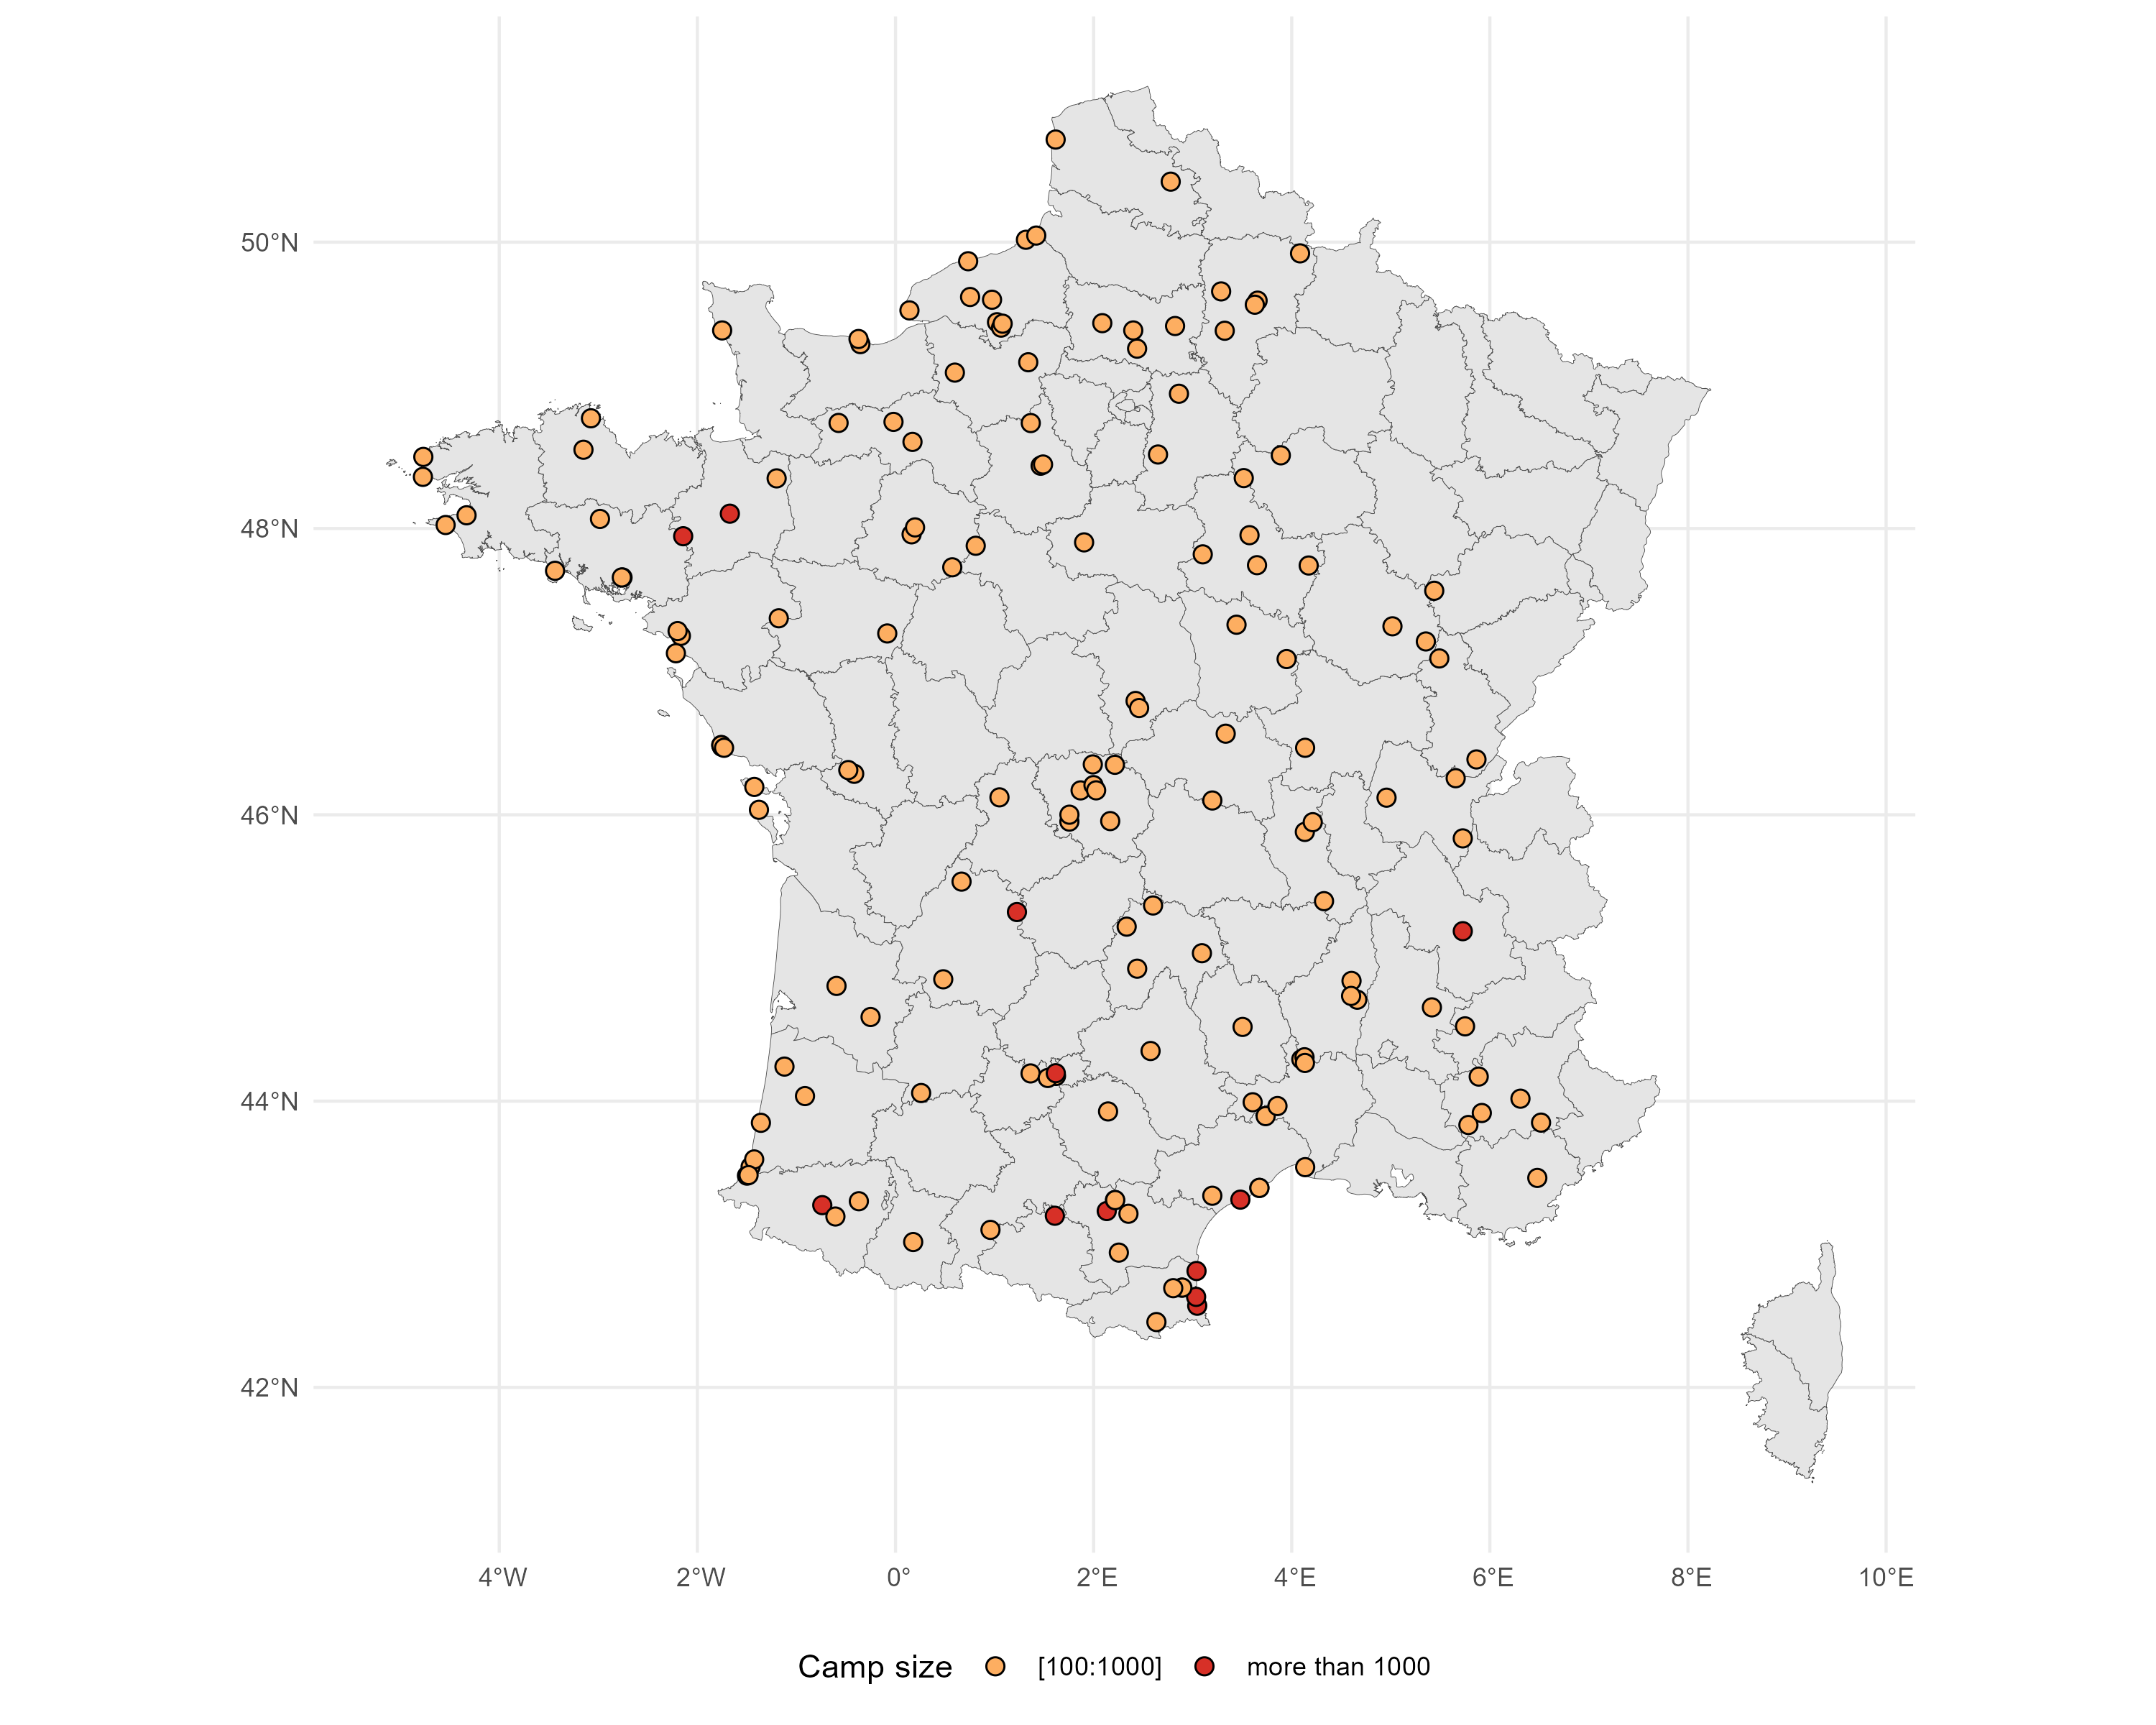
\includegraphics[width=\linewidth]{figures/descriptives/maps/map7.2.png}
        \subcaption{Medium and Large Size Camps}
    \end{minipage}
    \begin{minipage}{0.9\textwidth}
        \vspace{0.1in} 
        {\footnotesize Notes: The maps above display the locations of refugees camps across the French territory, per available information and size of camps. \par}
    \end{minipage}
\end{figure}




Table \ref{table:balance} reports balance statistics for the variables that are most relevant to assessing potential selection in the French dispersion policy. Because refugee placement was negotiated with departmental and municipal authorities, one concern is that more left-leaning municipalities may have been more willing to receive refugees; we therefore compare pre-war political orientation using the 1936 legislative results \citep{piketty_histoire_2023}. A second concern is municipality size: larger communes might have had more administrative capacity or available facilities, so we test for differences in population levels using historical census data \citep{insee_pop_hist_comm}. Another potential source of bias concerns the presence of other immigrant groups as the authorities may have avoided sending Spanish refugees to municipalities that had already received previous waves of foreigners. Because no city-level data on the share of the foreign population exist for this period, we approximate pre-existing immigrant presence using surname information from death records \citep{insee_deces_2025}. We identify French individuals with Spanish, Italian, or Portuguese surnames and recover their municipality of birth. From the same source, we also construct the share of women aged over twenty-one among the total population in the same age range. Balance in this measure is key considering women became eligible to vote in 1945. This does not pose a concern as long as treated and control municipalities exhibit comparable demographic structures.

Housing availability may have been another potential determinant of camp locations so we include a measure of buildings constructed by 1939 \citep{insee1968logements}. The Ministry of the Interior explicitly encouraged cooperation with private organisations such as the Red Cross and local philanthropic associations so we incorporate a measure of associative activity based on the legal registry of organisations \citep{dila_journalofficiel_portal}. Finally, we include variables capturing geographic and economic structure—altitude, precipitation, and mining activity \citep{pauling2006,camino2021}. Together, these variables allow us to test whether treated and control municipalities differed along the observable dimensions that could plausibly have influenced camp placement under the 1939 dispersion system.

Overall, observable characteristics are broadly similar across the two groups. Treated municipalities exhibit slightly higher support for the SFIO and the PCF, higher share of people with Italian-surnames, higher presence of mines and buildings per capita. Meanwhile, absolute standardized differences are below the conventional threshold of 0.25 \citep{ImbensRubin2015}. The exception is population, what we account for considering as an outcome share of votes with respect to total number of votes. 

\begin{table}[h!]
    \centering
    \caption{Balance test for municipalities with and without camps}
    \resizebox{0.8\textwidth}{!}{
    % latex table generated in R 4.5.0 by xtable 1.8-4 package
% Fri Mar  6 12:14:41 2026
\begin{tabular}{lrrrrr}
  \toprule
Variable & Mean Treated & SD Treated & Mean Control & SD Control & Abs. Norm. Diff \\ 
  \midrule
SFIO & 0.194 & 0.205 & 0.177 & 0.189 & 0.082 \\ 
  RAD SOC & 0.189 & 0.205 & 0.198 & 0.209 & 0.046 \\ 
  DIV & 0.001 & 0.008 & 0.006 & 0.053 & 0.108 \\ 
  FR URD & 0.133 & 0.235 & 0.159 & 0.252 & 0.108 \\ 
  DVG & 0.004 & 0.040 & 0.002 & 0.028 & 0.057 \\ 
  PCF & 0.104 & 0.126 & 0.085 & 0.114 & 0.161 \\ 
  DVD & 0.018 & 0.091 & 0.015 & 0.084 & 0.034 \\ 
  AGR & 0.009 & 0.052 & 0.019 & 0.080 & 0.148 \\ 
  USR & 0.071 & 0.151 & 0.069 & 0.154 & 0.013 \\ 
  AD & 0.277 & 0.245 & 0.270 & 0.271 & 0.028 \\ 
  Italian-origin surnames (share) & 0.167 & 0.042 & 0.165 & 0.064 & 0.022 \\ 
  Spanish-origin surname (share) & 0.064 & 0.038 & 0.064 & 0.048 & 0.000 \\ 
  Portuguese-origin surname (share) & 0.002 & 0.004 & 0.002 & 0.007 & 0.039 \\ 
  Associations (per capita) & 0.003 & 0.003 & 0.004 & 0.007 & 0.227 \\ 
  Presence of mines & 0.115 & 0.319 & 0.085 & 0.279 & 0.100 \\ 
  Buildings per capita & 0.319 & 0.113 & 0.308 & 0.097 & 0.109 \\ 
  Altitude & 262.237 & 279.532 & 279.950 & 296.883 & 0.061 \\ 
  Population & 3925.122 & 14860.324 & 941.338 & 3854.599 & 0.275 \\ 
  Mean rainfall & 807.804 & 160.548 & 817.462 & 163.060 & 0.060 \\ 
  WWI death rate & 3.776 & 1.370 & 4.093 & 3.440 & 0.121 \\ 
  Share of women 1936 & 0.575 & 0.043 & 0.571 & 0.062 & 0.060 \\ 
  Share of women 1945 & 0.555 & 0.035 & 0.553 & 0.052 & 0.047 \\ 
   \bottomrule
\end{tabular}
}
    \label{table:balance}
\begin{minipage}{0.8\textwidth}
        \vspace{0.5em}
\footnotesize
\textit{Notes:} All variables are measured before 1939, except for buildings per capita that includes 1939 due to limitations in the census. Electoral outcomes correspond to the 1936 legislative elections. 
\end{minipage}

\end{table}


\section{Empirical Strategy}\label{sec:empirical_strategy}


Studying the political effects of immigration requires addressing endogeneity issues that are intrinsic to the topic of immigration: immigrants typically self-select into locations based on local factors related to political outcomes. This historical episode offers a unique opportunity to study the local impact of refugee exposure in a quasi-experimental setting. Because the internment camps were established under severe time constraints, their locations were shaped mainly by logistical considerations. We estimate the effect of exposure to refugee camps on political outcomes using a two-way fixed-effects specification. 

Traditionally, the standard estimator for spatially targeted treatments with geocoded microdata compares units located immediately next to the treated area with units situated slightly farther away. The motivation is that, because treated and control units lie in close physical proximity, they should be exposed to similar time-varying shocks. However, this approach depends on correctly identifying the spatial extent of treatment effects. If the treated ring is defined too narrowly, units in the control ring may still be affected by the treatment, so changes among “controls” no longer recover the counterfactual trend. Conversely, if the treated ring is defined too broadly, untreated units are averaged into the “treated” group, attenuating estimates toward zero. 

\citet{butts_difference--differences_2023} formalize how to adjust the two-way fixed-effects estimator to account for such spatial spillovers. Using his approach, we construct concentric 5-kilometre rings to capture municipalities at varying distances from the refugee camps. \Cref{fig:map_example_methodology} in the Annex shows as an example the department of Gers. This spatial design allows us to identify the treatment effect separately for each ring in the difference-in-differences framework.

\begin{equation}\label{equation:political}
y_{it} = \tau D_{it}
+ \sum_{j=1}^{n} (1 - D_{it}) Ring_{ij}
+ X_{it}'\beta
+ \mu_i + \lambda_{t \times d} + \varepsilon_{it}
\end{equation}


In this specification, $y_{it}$ denotes the share of vote for a particular party in municipality $i$ at time $t$. The variable $D_{it}$ equals 1 for municipalities that are 1 kilometre close to a refugee camp in periods after treatment, and 0 otherwise. The term $\sum_{j=1}^{n} (1 - D_{it})\, Ring_{ij}$ introduces a set of distance rings, where $Ring_{ij}$ equals 1 if municipality $i$ lies in ring $j$. The rings used in the specification are 2--5 km, 5--10 km, 10--15 km, 15--20 km, and 20--25 km from the nearest camp. The control group consists of municipalities located within 40 km. The factor $(1 - D_{it})$ ensures that spillover effects are estimated only among non-treated municipalities. The coefficient $\tau$ captures the direct effect of hosting a camp, while the coefficients on the ring indicators measure the average spillover effects at different distances. The vector $X_{it}$ includes time-varying control variables, specifically total municipal population. The term $\mu_i$ represents municipality fixed effects, and $\lambda_{t \times d}$ denotes year fixed effects interacted with department fixed effects to absorb common shocks at the department-year level. Standard errors are clustered at the municipality level. 













\section{Preliminary Results}\label{sec:results}


\subsection{Results in voting}

COMMENT TURNOUT 

\begin{table}[h!]
    \centering
    \caption{Impact of refugee camp exposure on turnout}
    \resizebox{0.6\textwidth}{!}{\begingroup
\centering
\begin{tabular}{lcc}
   \toprule
                                 & Spillovers     & Control as 20-40km \\   
                                 & (1)            & (2)\\  
   \midrule 
   Within 1 km                   & 0.0197$^{***}$ & 0.0256$^{***}$\\   
                                 & (0.0025)       & (0.0031)\\   
   Ring 5                        & 0.0057$^{***}$ &   \\   
                                 & (0.0019)       &   \\   
   Ring 10                       & 0.0039$^{**}$  &   \\   
                                 & (0.0018)       &   \\   
   Ring 15                       & 0.0009         &   \\   
                                 & (0.0018)       &   \\   
   Ring 20                       & -0.0002        &   \\   
                                 & (0.0018)       &   \\   
   Ring 25                       & -0.0023        &   \\   
                                 & (0.0019)       &   \\   
   Ring 30                       & -0.0025        &   \\   
                                 & (0.0018)       &   \\   
    \\
   R$^2$                         & 0.517          & 0.566\\  
   Observations                  & 262,080        & 74,954\\  
    \\
   Municipality fixed effects & $\checkmark$   & $\checkmark$\\   
   Time-Reg fixed effects     & $\checkmark$   & $\checkmark$\\   
   \bottomrule
\end{tabular}
\par\endgroup
}
    \label{table:communist_results}
        \vspace{0.5em}
        \begin{minipage}{0.6\textwidth}
            \footnotesize
            Note: In the first column, we estimate \cref{equation:political}. In the second column, the control group are those within 20-40km.  Standard errors (SE) are clustered at the municipality level. *** p$<$0.01, ** p$<$0.05, * p$<$0.1.
        \end{minipage}
\end{table}

\begin{figure}[htbp]
  \centering
  \caption{Impact of Refugee Camp Exposure on turnout - ring estimations}
  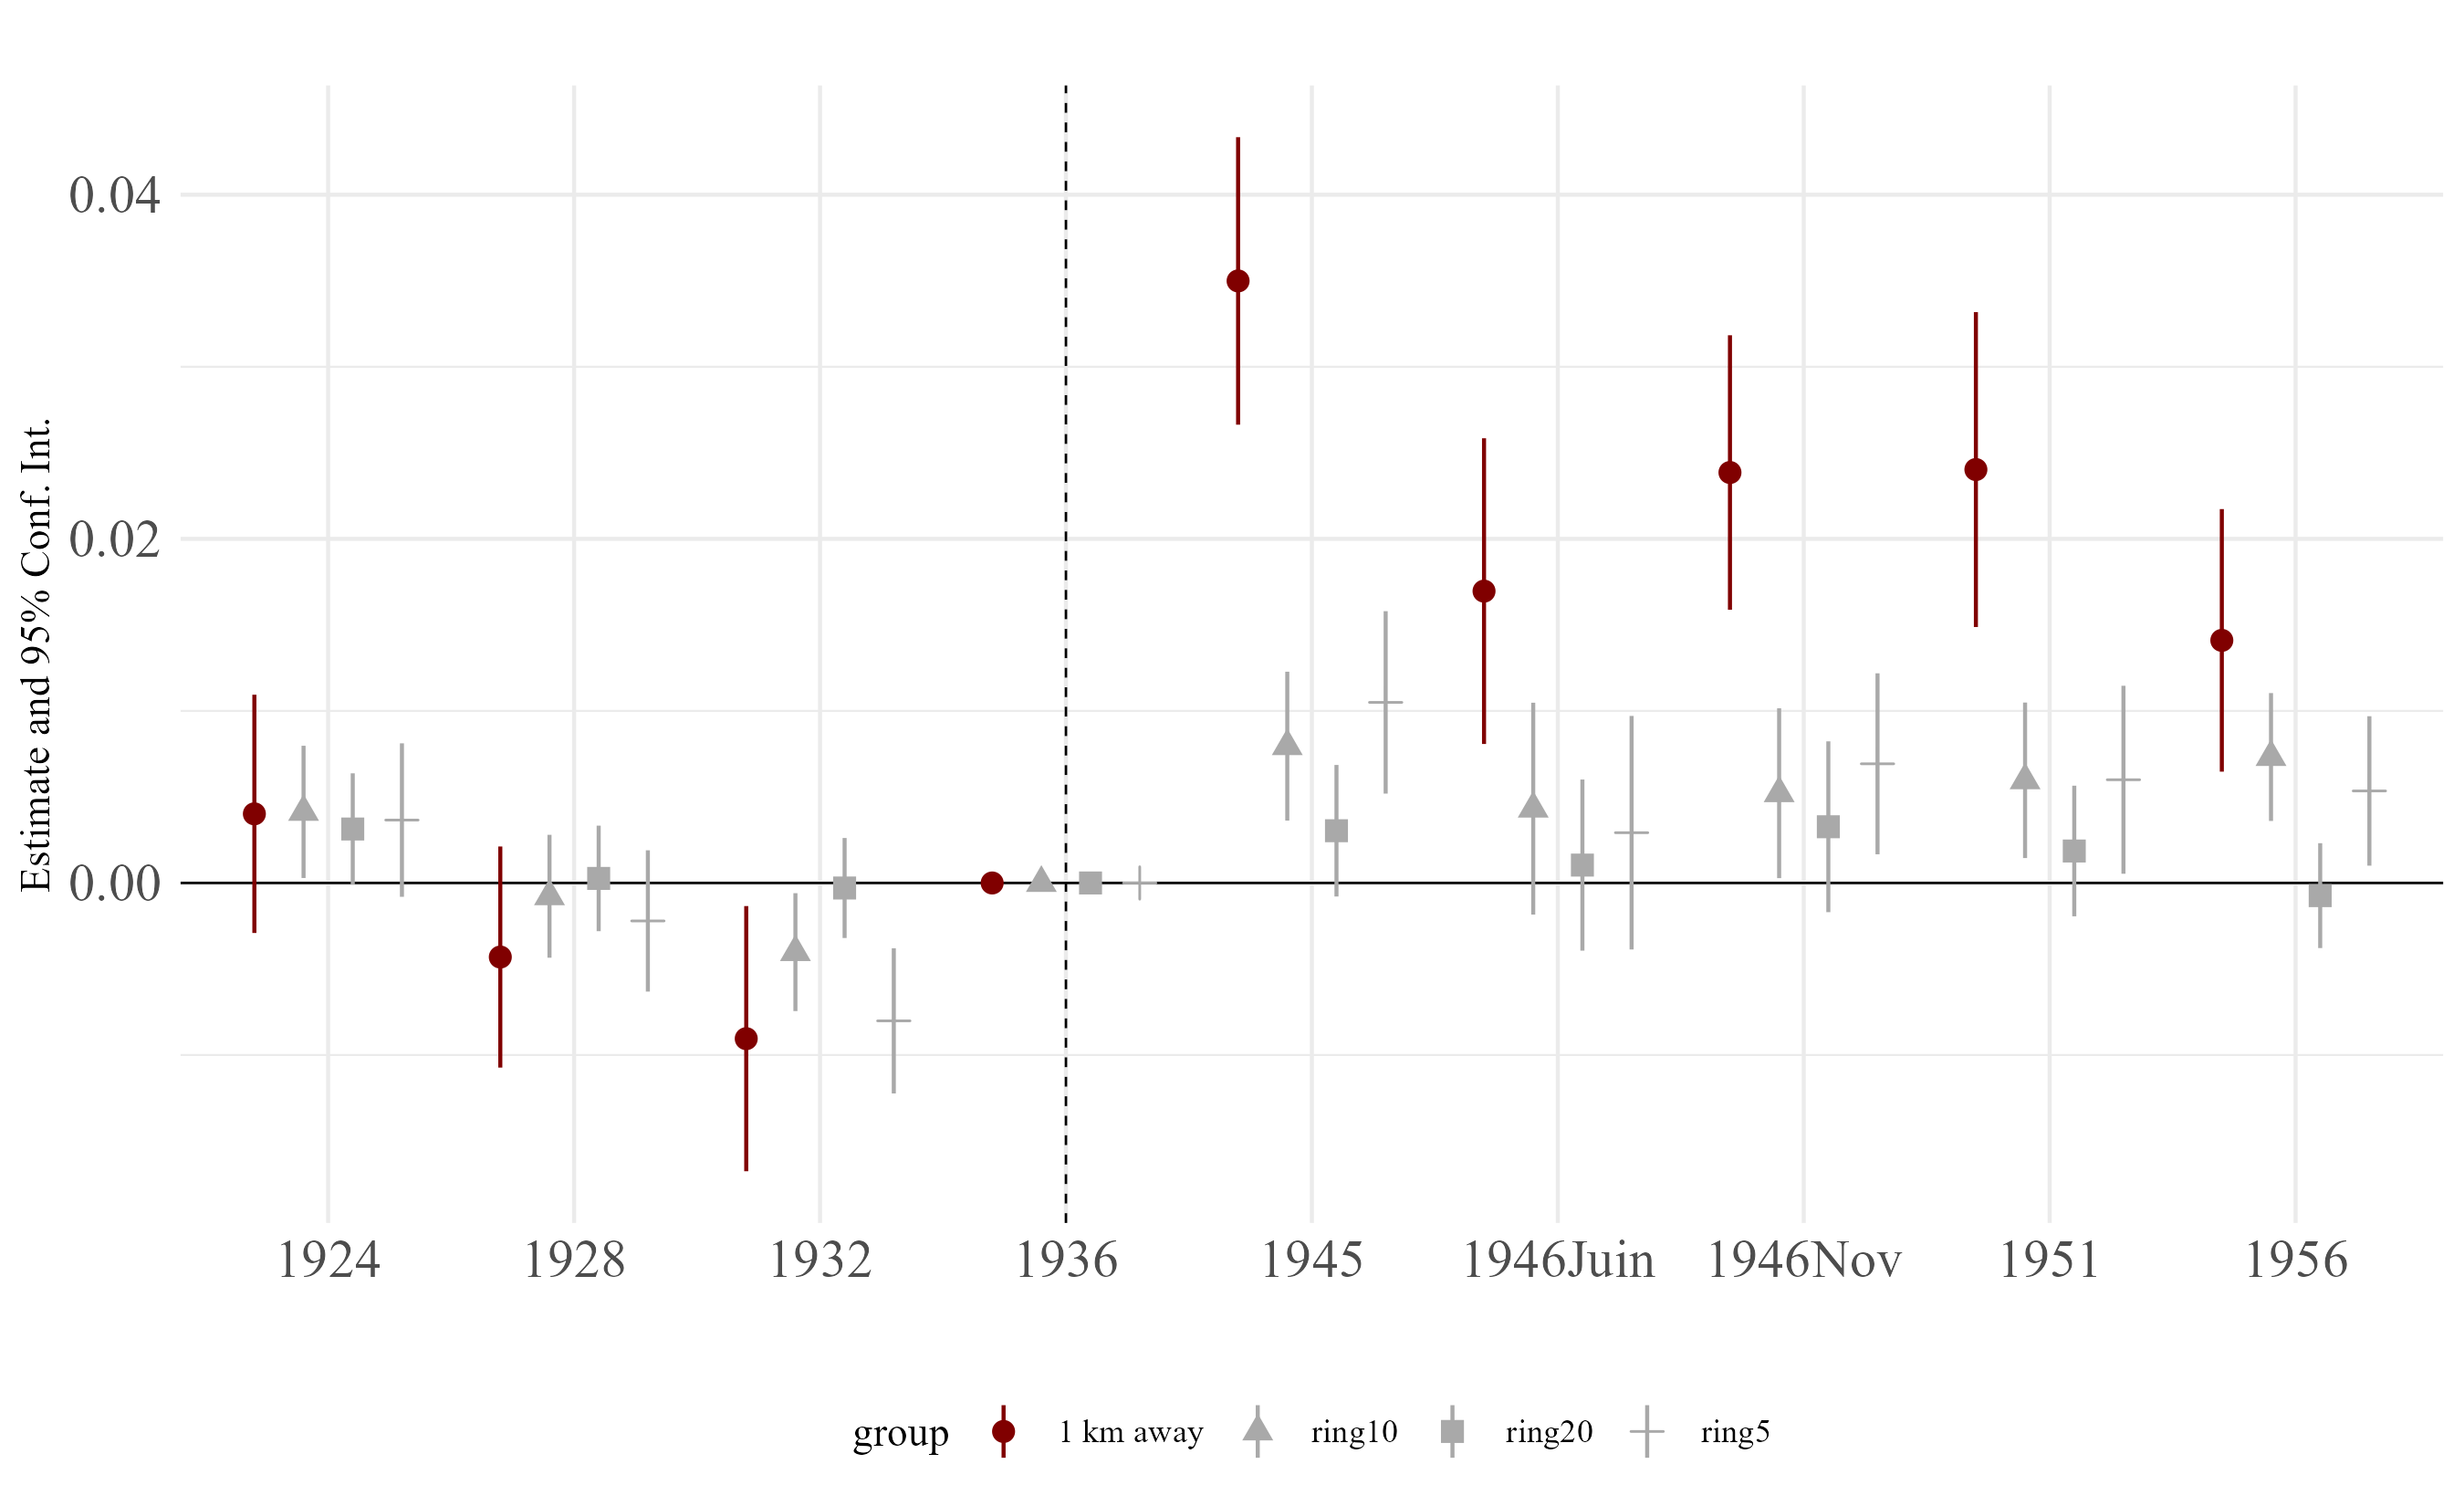
\includegraphics[width=0.8\linewidth]{figures/results/political/turnout_event_study.png}
  \label{fig:SFIO_all}
   \begin{minipage}{0.7\textwidth}
        \vspace{0.5em}
        {\footnotesize Notes: This graph reports the estimates from \cref{equation:political}, where the coefficient for each ring is estimated using municipalities located 20–40 km away as the control group. Error bars plot the interval confidence at 95\%. Standard errors are clustered at the municipality level.\par}
        \end{minipage}
\end{figure}


We examine how exposure to refugee camps affected political outcomes. The analysis focuses on the vote share of the SFIO (“Section Fran\c{c}aise de l’Internationale Ouvri`ere”), the socialist party, because it is the only political group that spans the entire period under study and it does not experience major ideological transformations before and after our treatment. \Cref{table:SFIO_results} shows several difference-in-differences specifications to examine the effect of hosting a camp on the share of votes of the socialist party. In the first column, we compare treated municipalities (those within 1 km) with cities within 40 km as controls. In the second column, we compare units treated units to those further away (within 20 to 40 km). The third column shows the coefficients of \Cref{equation:political}, which accounts for spatial spillovers by including a set of concentric circles. The results show a significant reduction in the share of votes for the socialist party in all the specifications. In our preferred specification, municipalities exposed to a camp have on average 2,7 percentage points lower vote share for the socialist party, which represents a 10\% reduction with respect to the pretreatment mean. 

\begin{table}[h!]
    \centering
    \caption{Impact of refugee camp exposure on socialist vote share}
    \resizebox{0.6\textwidth}{!}{\begingroup
\centering
\begin{tabular}{lcc}
   \toprule
                                 & Spillovers      & Control as 20-40km \\   
                                 & (1)             & (2)\\  
   \midrule 
   Within 1 km                   & -0.0150$^{***}$ & -0.0283$^{***}$\\   
                                 & (0.0038)        & (0.0055)\\   
   Ring 5                        & -0.0064$^{**}$  &   \\   
                                 & (0.0030)        &   \\   
   Ring 10                       & -0.0029         &   \\   
                                 & (0.0029)        &   \\   
   Ring 15                       & -0.0038         &   \\   
                                 & (0.0029)        &   \\   
   Ring 20                       & 0.0019          &   \\   
                                 & (0.0028)        &   \\   
   Ring 25                       & 0.0068$^{**}$   &   \\   
                                 & (0.0028)        &   \\   
   Ring 30                       & 0.0017          &   \\   
                                 & (0.0029)        &   \\   
    \\
   R$^2$                         & 0.779           & 0.789\\  
   Observations                  & 261,841         & 74,781\\  
    \\
   Municipality fixed effects & $\checkmark$    & $\checkmark$\\   
   Time-Reg fixed effects     & $\checkmark$    & $\checkmark$\\   
   \bottomrule
\end{tabular}
\par\endgroup
}
    \label{table:SFIO_results}
        \begin{minipage}{0.6\textwidth}
        \vspace{0.5em}
            \footnotesize
            Note: In the first column, we estimate \cref{equation:political}. In the second column, the control group are those within 20-40km.  Standard errors (SE) are clustered at the municipality level. *** p$<$0.01, ** p$<$0.05, * p$<$0.1.
        \end{minipage}
\end{table}

\Cref{fig:SFIO_all} shows the results of the event study by buffer size - within 1 km, within 10 km away and 20 km - considering the municipalities within 40 km as control group. Before the war, the coefficients suggest no systematic pre-trend for the estimations of municipalities that are nearby camps. After 1945, however, municipalities exposed to refugee camps record a persistent decline in SFIO support, with estimates becoming increasingly negative through the 1950s. This pattern is consistent with a political backlash: exposure to the camps may have deteriorated the image of the socialist left, historically associated with solidarity and internationalism, eroding their electoral support. The figure also shows significant spillovers effects to nearby municipalities. For municipalities within 30 km, the effects vanish because the buffer increasingly draws in control municipalities. 


\begin{figure}[htbp]
  \centering
  \caption{Impact of Refugee Camp Exposure on socialist vote share - ring estimations}
  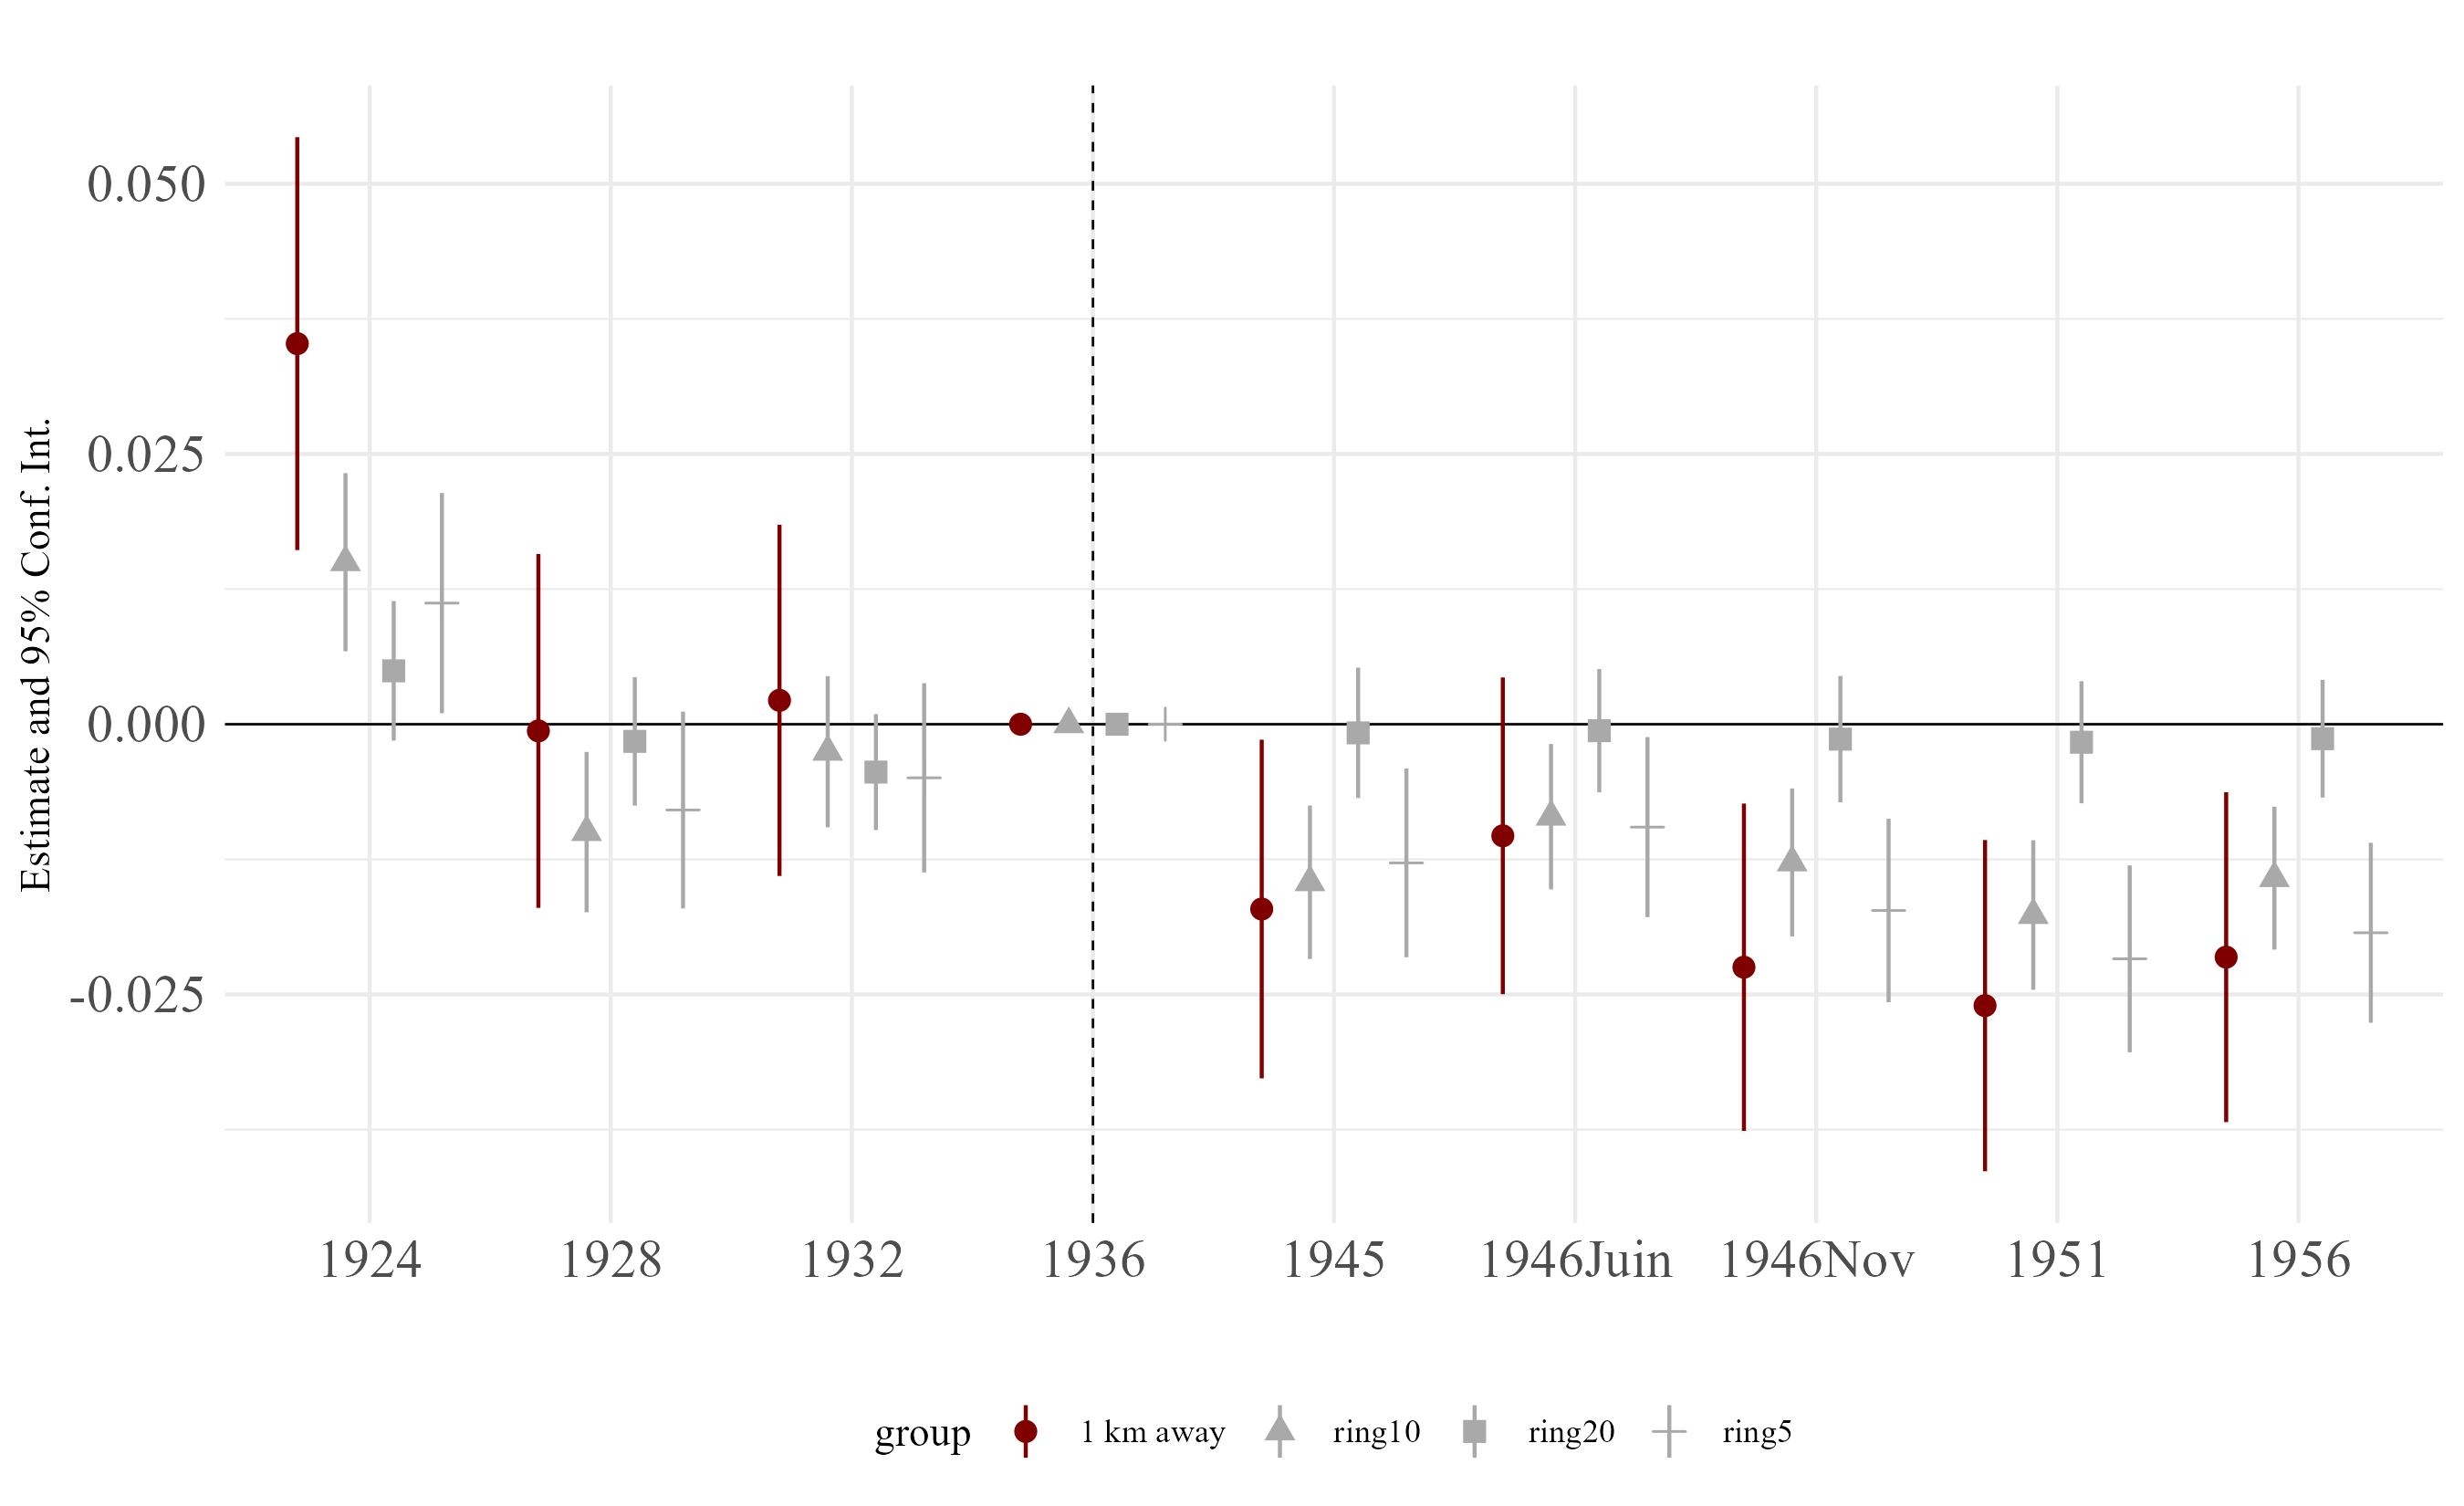
\includegraphics[width=0.8\linewidth]{figures/results/political/pvoixSFIO_event_study.png}
  \label{fig:SFIO_all}
   \begin{minipage}{0.7\textwidth}
        \vspace{0.5em}
        {\footnotesize Notes: This graph reports the estimates from \cref{equation:political}, where the coefficient for each ring is estimated using municipalities located 20–40 km away as the control group. Error bars plot the interval confidence at 95\%. Standard errors are clustered at the municipality level.\par}
        \end{minipage}
\end{figure}


Right-wing parties are not comparable before and after the shock because there is no single party that exists continuously throughout the entire period of analysis.\footnote{Throughout the interwar and post-war years, the composition of the French right changed substantially. Key parties present before the war—such as the Fédération républicaine or the Alliance démocratique—either disappeared, were absorbed, or were replaced after 1945 by entirely new formations like the MRP or, later, the Gaullist RPF.} We include the results on right-wing support in the Annex using the aggregation done by \citet{piketty_histoire_2023}, which shows a positive and significant effect, in line with our main results. 


\Cref{table:communist_results} extends this analysis by examining responses at the far left of the spectrum, focusing on the Communist Party. Because the PCF first appears in the 1924 legislative elections, caution is required due to limited pre-treatment periods. Nonetheless, once spatial spillovers are accounted for, we find that exposure to the camps increases the PCF vote share: municipalities within 1 km record an increase of roughly 1.6 percentage points or 15\% increase with respect to the pretreatment mean. The effects gradually decline toward zero as distance increases. 


\begin{table}[h!]
    \centering
    \caption{Impact of refugee camp exposure the communist vote shares}
    \resizebox{0.6\textwidth}{!}{\begingroup
\centering
\begin{tabular}{lcc}
   \toprule
                                 & Spillovers     & Control as 20-40km \\   
                                 & (1)            & (2)\\  
   \midrule 
   Within 1 km                   & 0.0166$^{***}$ & 0.0238$^{***}$\\   
                                 & (0.0033)       & (0.0050)\\   
   Ring 5                        & 0.0175$^{***}$ &   \\   
                                 & (0.0027)       &   \\   
   Ring 10                       & 0.0140$^{***}$ &   \\   
                                 & (0.0026)       &   \\   
   Ring 15                       & 0.0131$^{***}$ &   \\   
                                 & (0.0025)       &   \\   
   Ring 20                       & 0.0104$^{***}$ &   \\   
                                 & (0.0025)       &   \\   
   Ring 25                       & 0.0048$^{*}$   &   \\   
                                 & (0.0025)       &   \\   
   Ring 30                       & -0.0018        &   \\   
                                 & (0.0025)       &   \\   
    \\
   R$^2$                         & 0.823          & 0.831\\  
   Observations                  & 261,841        & 74,781\\  
    \\
   Municipality fixed effects & $\checkmark$   & $\checkmark$\\   
   Time-Reg fixed effects     & $\checkmark$   & $\checkmark$\\   
   \bottomrule
\end{tabular}
\par\endgroup
}
    \label{table:communist_results}
    \vspace{0.5em}
        \begin{minipage}{0.6\textwidth}
            \footnotesize
            Note: In the first column, we estimate \cref{equation:political}. In the second column, the control group are those within 20-40km.  Standard errors (SE) are clustered at the municipality level. *** p$<$0.01, ** p$<$0.05, * p$<$0.1.
        \end{minipage}
\end{table}

COMMENT EVENT STUDY 

\begin{figure}[htbp]
  \centering
  \caption{Impact of refugee camp exposure the communist vote shares - ring estimations}
  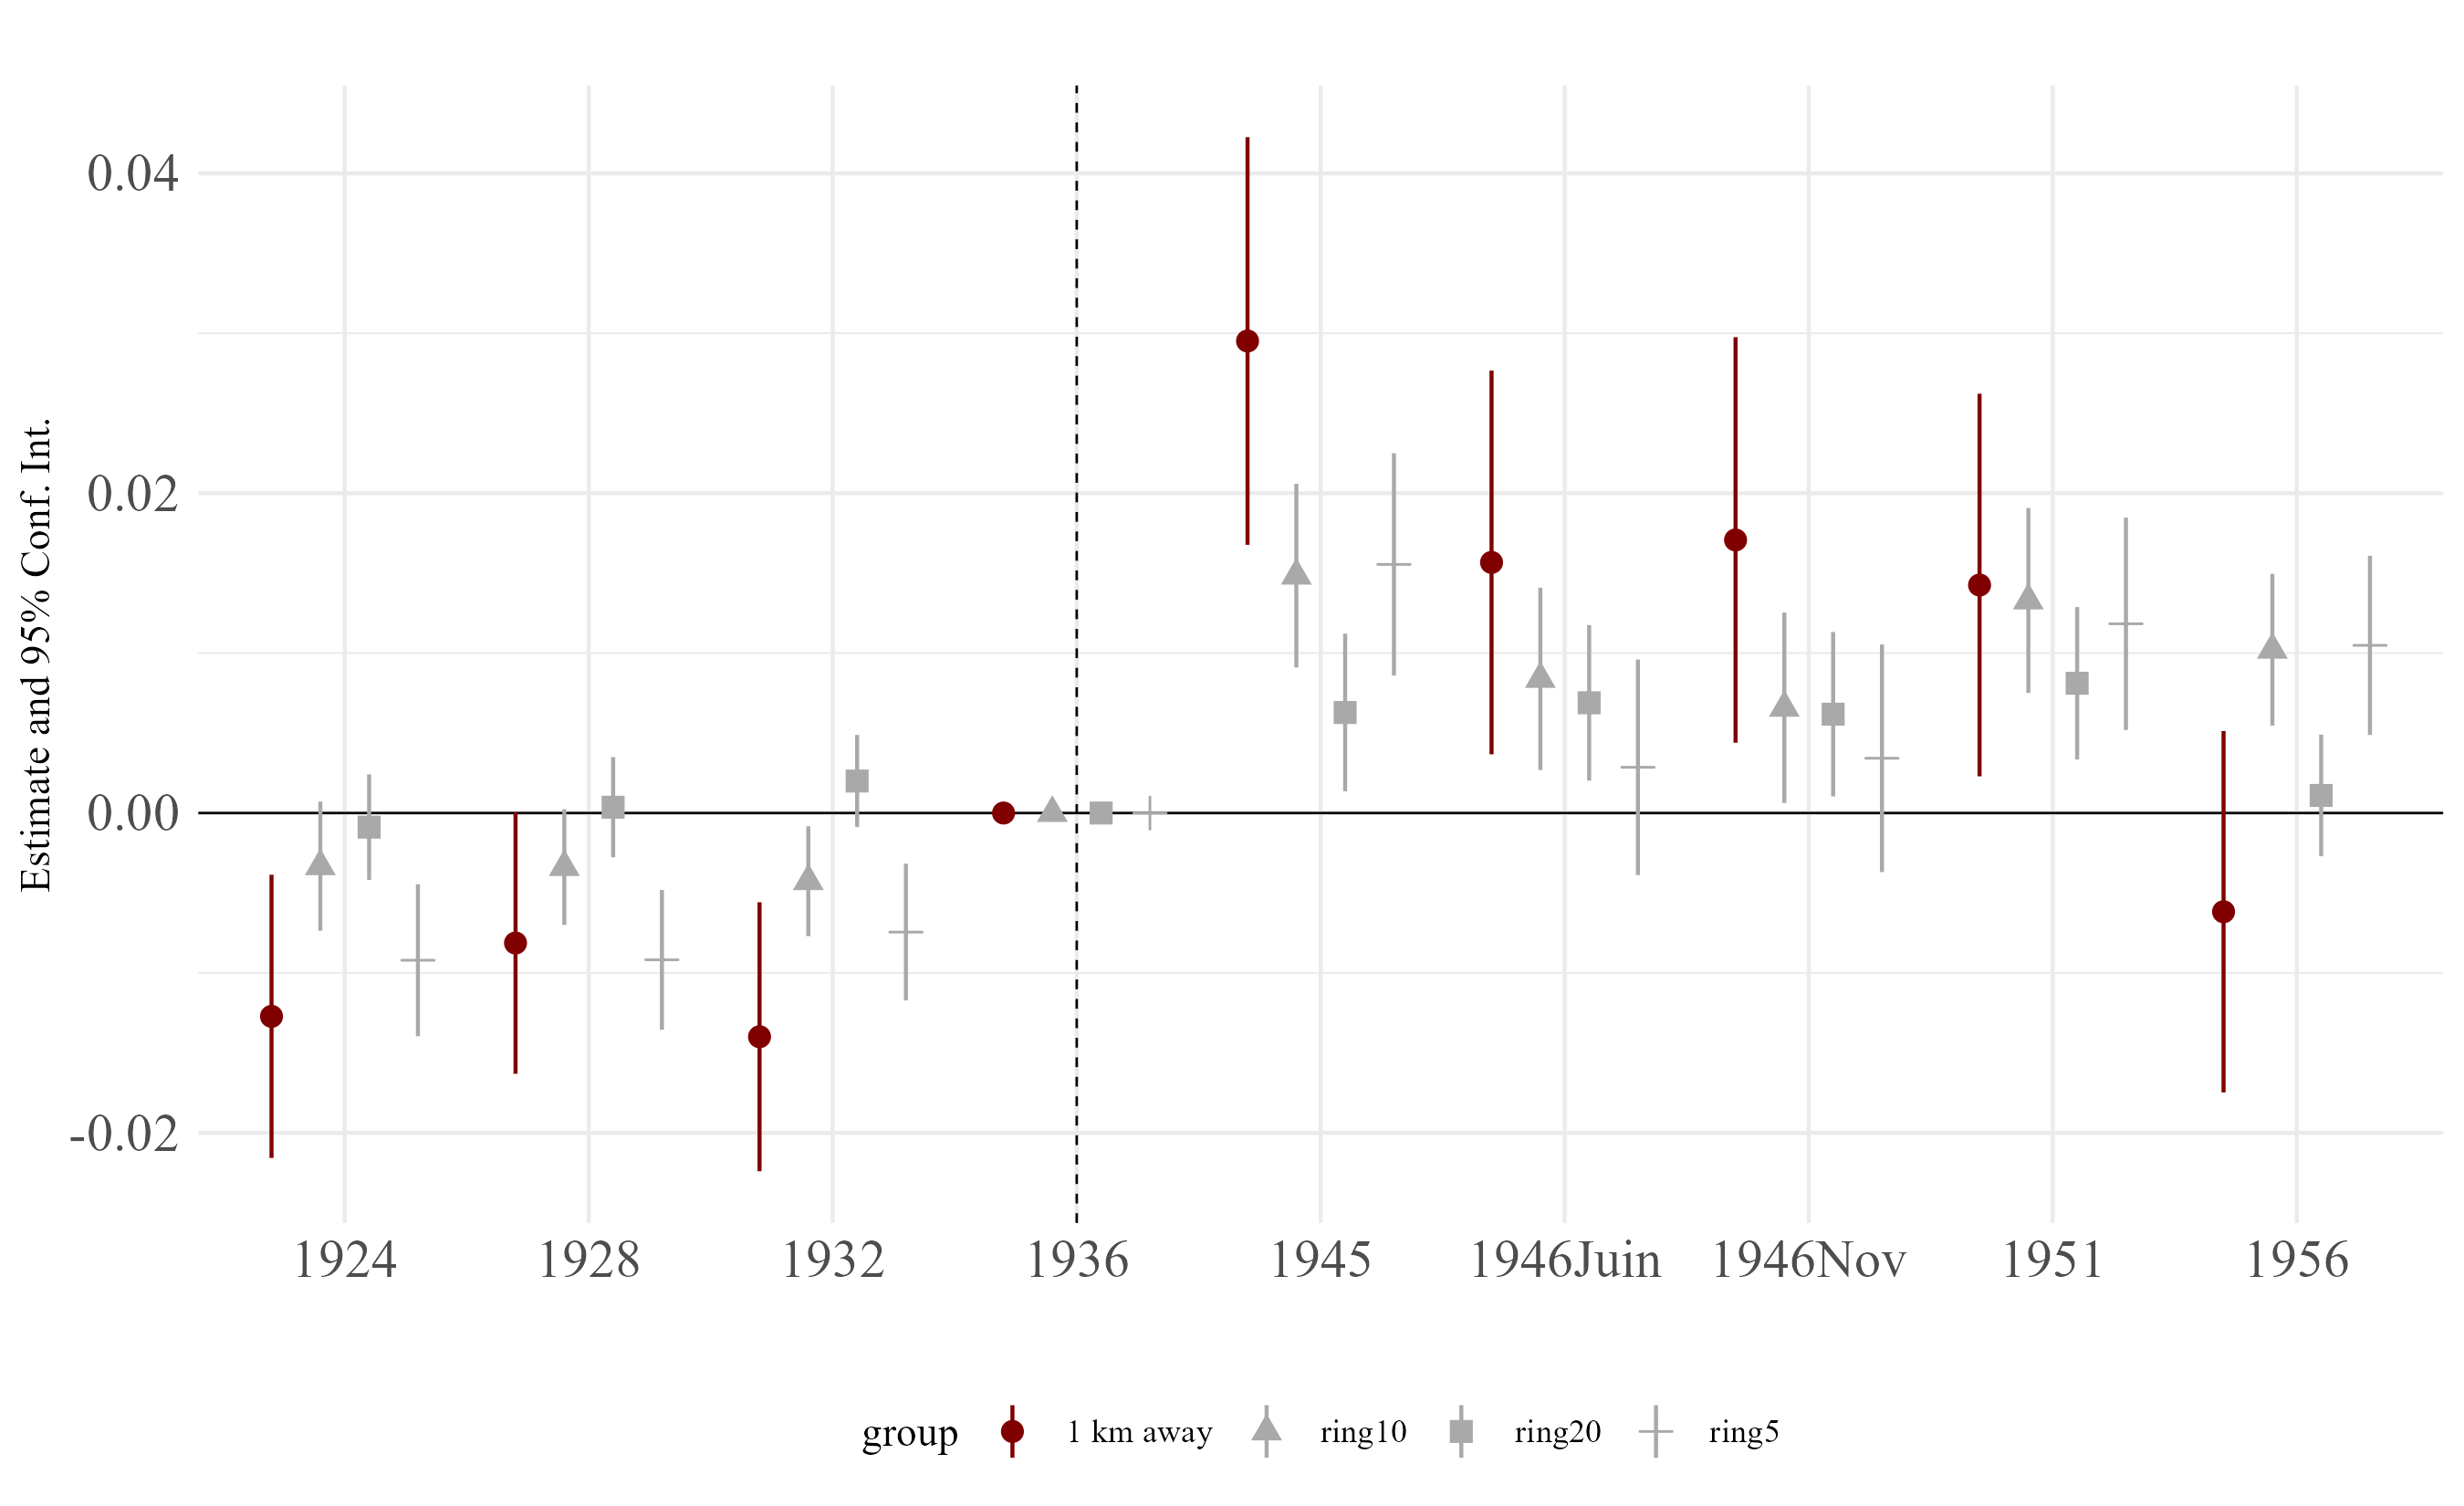
\includegraphics[width=0.8\linewidth]{figures/results/political/pvoixPCF_event_study.png}
  \label{fig:SFIO_all}
   \begin{minipage}{0.7\textwidth}
        \vspace{0.5em}
        {\footnotesize Notes: This graph reports the estimates from \cref{equation:political}, where the coefficient for each ring is estimated using municipalities located 20–40 km away as the control group. Error bars plot the interval confidence at 95\%. Standard errors are clustered at the municipality level.\par}
        \end{minipage}
\end{figure}


We argue that the political effect that we document depends on the size of the camps the local population are exposed to. The effects of refugees camps by the size of the camp are jointly estimated in the same regression. In \autoref{fig:PCF_SFIO_camps_sizes}, we show the ATT on the share of votes for the SFIO and the PCF within a buffer of 1 kilometre of exposure, depending on the size of the camps they are exposed as defined by the quartile in terms of refugees population\footnote{See \autoref{fig:bars_camps_sizes} for the definition of the quartiles.}. The exposure to a camps with a refugee population lower than 20 individuals does not have any significant effect on the vote for the communist party after the war, and is slight significant for the socialist party. Overall, we observe a positive correlation between the size of the camp population and both the magnitude and statistical significance of the effect that we measure. EVENT STUDIES IN THE ANNEX. 



\begin{figure}[h!]
  \centering
  \caption{Impact on the Share of Votes, per Size of Camps}
  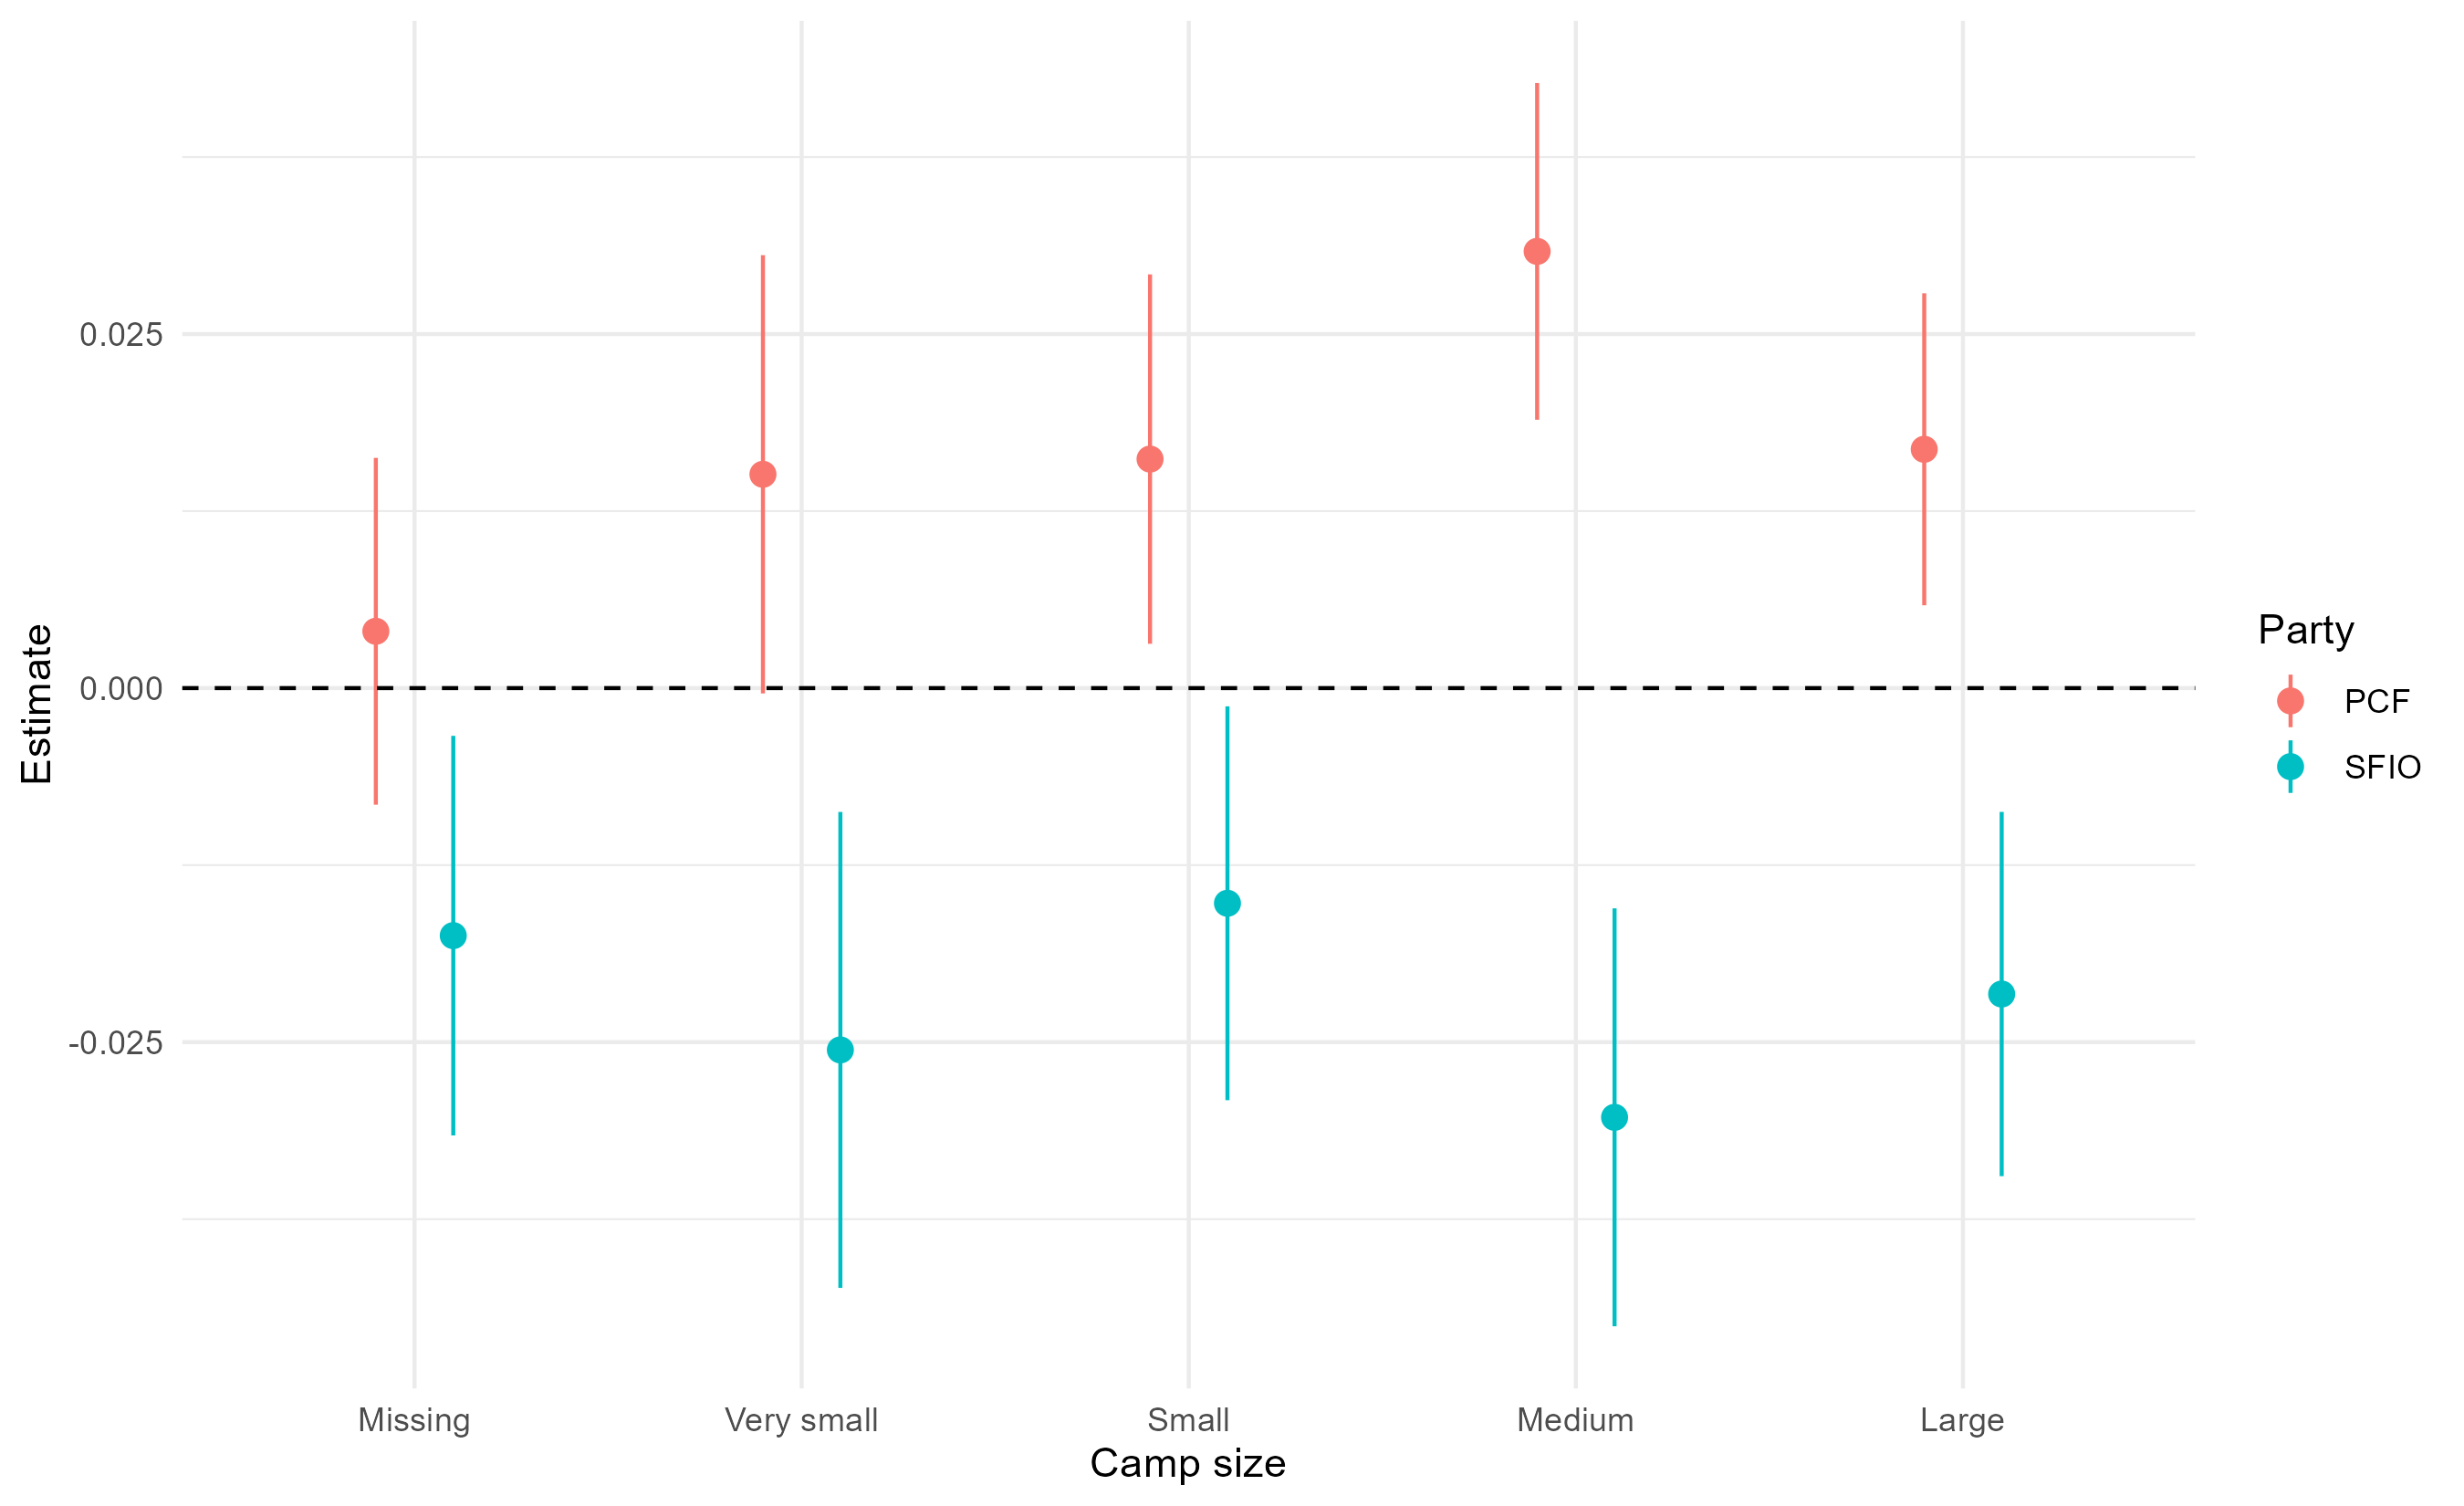
\includegraphics[width=0.8\linewidth]{figures/results/political/effect_size.png}
  \label{fig:PCF_SFIO_camps_sizes}
   \begin{minipage}{0.7\textwidth}
   \vspace{0.1in} 
        {\tiny This graph reports the jointly estimated average treatment effects of the different camps, by size, on vote shares for the Socialists (SFIO) and the Communists (PCF). The control municipalities are those within 20-40 km. The distribution of the population camps and their categorization per population quartiles is reported in \autoref{fig:bars_camps_sizes}.Error bars plot the interval confidence at 95\%. Standard errors are clustered at the department level.\par}
        \end{minipage}
\end{figure}



\subsection{Results in mobilization}


We now examine whether the effects differ across the political spectrum to explore political polarization and diffusion of ideas. We explore the relationship between the location of the camps and the resistance movement to explore the effect on the behaviour among a politically selective minority rather than population-wide responses. These measures reflect actions taken by individuals who were already highly engaged in political or civic life. Several organizations were especially active in mobilizing around the arrival of the Spanish refugees: the General Confederation of Labour (CGT), professional unions and cooperative federations. Members of these groups were more likely to interact directly with the Republican refugees. If ideas brought by the refugees diffused locally, politically active individuals are the ones most likely to internalize and act upon them. Any diffusion mechanism would therefore be expected to appear at the political extremes, where responses may diverge from those of the average voter.

%collaborators: and \Cref{fig:collabos} 
%in the case of resistance, whereas it remains significant up to 15 km for collaboration. This pattern cannot be explained by political selection in the siting of the camps. Instead, it aligns with increasing political polarization in municipalities closer to the camps. 

\Cref{fig:resistants} displays coefficient estimates by distance to the nearest refugee camp, with each point corresponding to a separate regression. The results indicate a positive association between proximity to a camp and resistance participation. This effect is concentrated within 3 km and disappears at larger distances. Within this radius, camp proximity is associated with an approximately 13\% increase in the expected number of individuals participating in the resistance, corresponding to about 1.5 additional individuals per municipality. This pattern is consistent with the results on the communist party, considering the links between the PCF and the resistance movement. 


\begin{figure}[htbp]
  \centering
    \caption{Effect of Refugee Camp Exposure on Resistance, by Distance}
  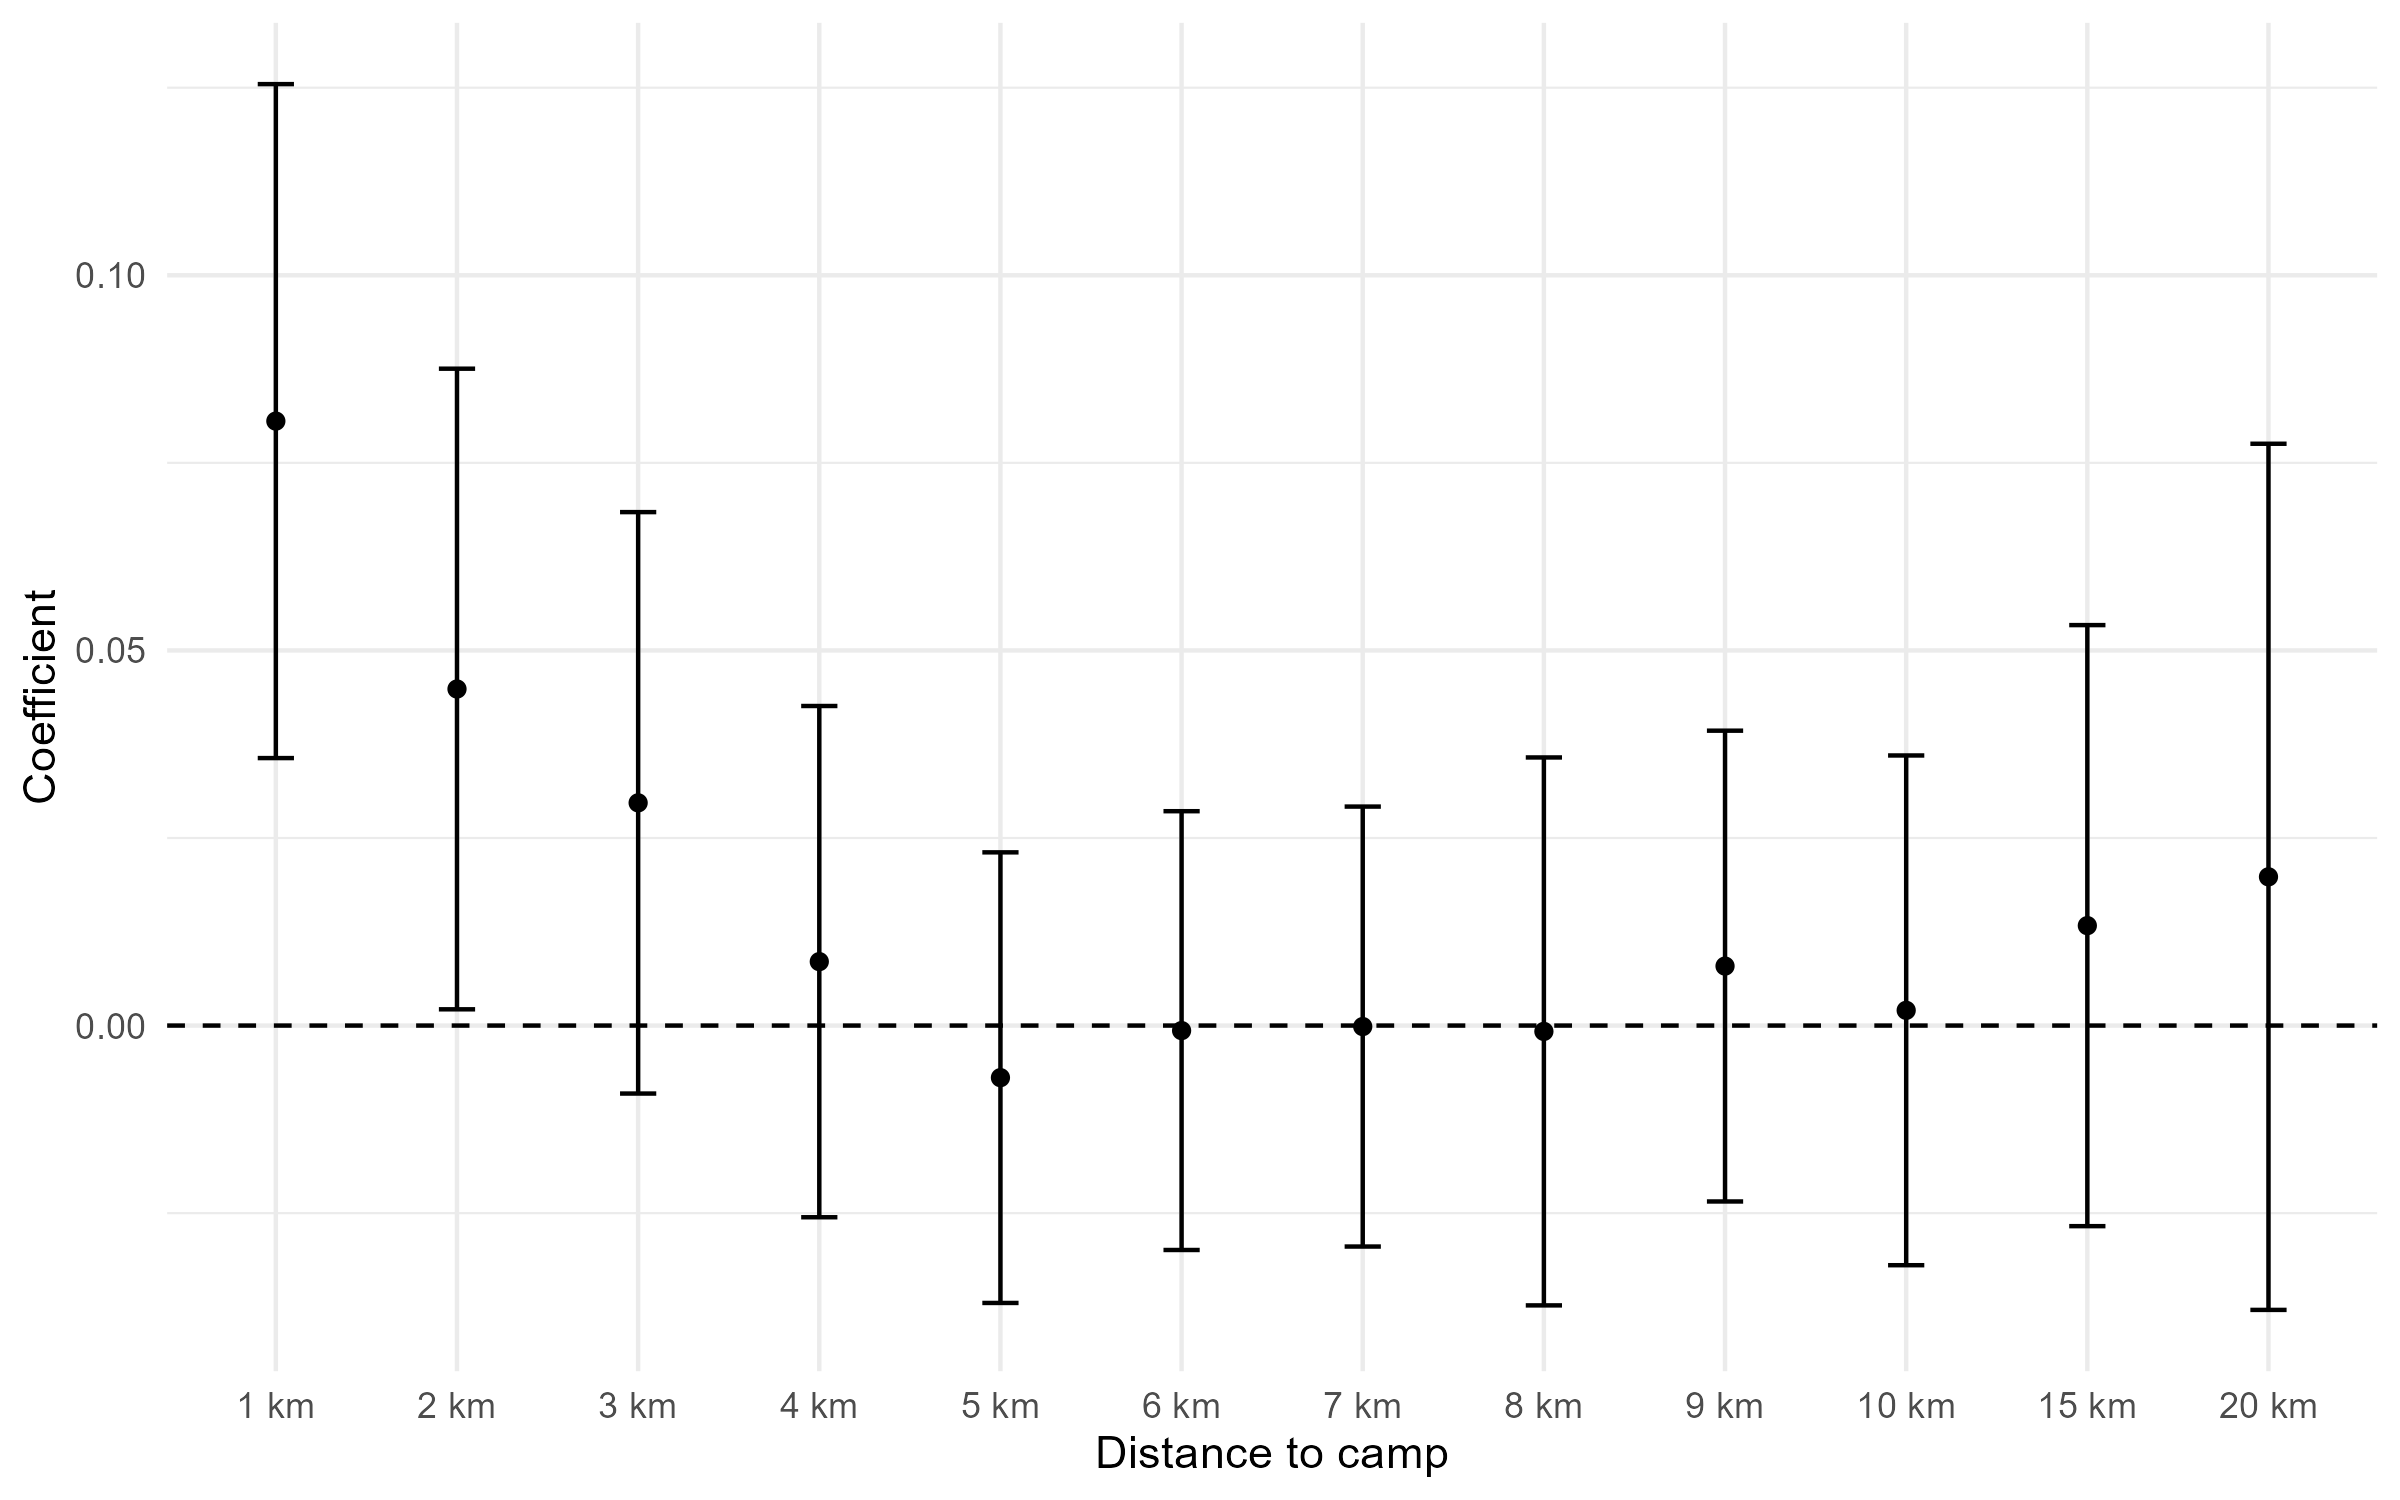
\includegraphics[width=0.8\linewidth]{figures/results/mobilisation/poisson_count_total.png}
  \label{fig:resistants}
   \begin{minipage}{0.8\textwidth}
        \vspace{0.1in} 
        {\footnotesize Notes: This graph reports the estimates of Poisson regressions on the number of resistants against Nazi Occupation. Error bars plot the interval confidence at 95\%. Standard errors are clustered to account for spatial correlation using \citet{conley_gmm_1999} (100 km). All specifications include region fixed effects and a set of controls—surname-based birthplace composition, altitude, mining activity, buildings per capita, average rainfall and the share of votes for the political parties of the 1936 legislative elections —and include a population offset.\par}
        \end{minipage}
\end{figure}

\begin{figure}[htbp]
  \centering
    \caption{Effect of Refugee Camp Exposure on Resistance, by size of the camp}
  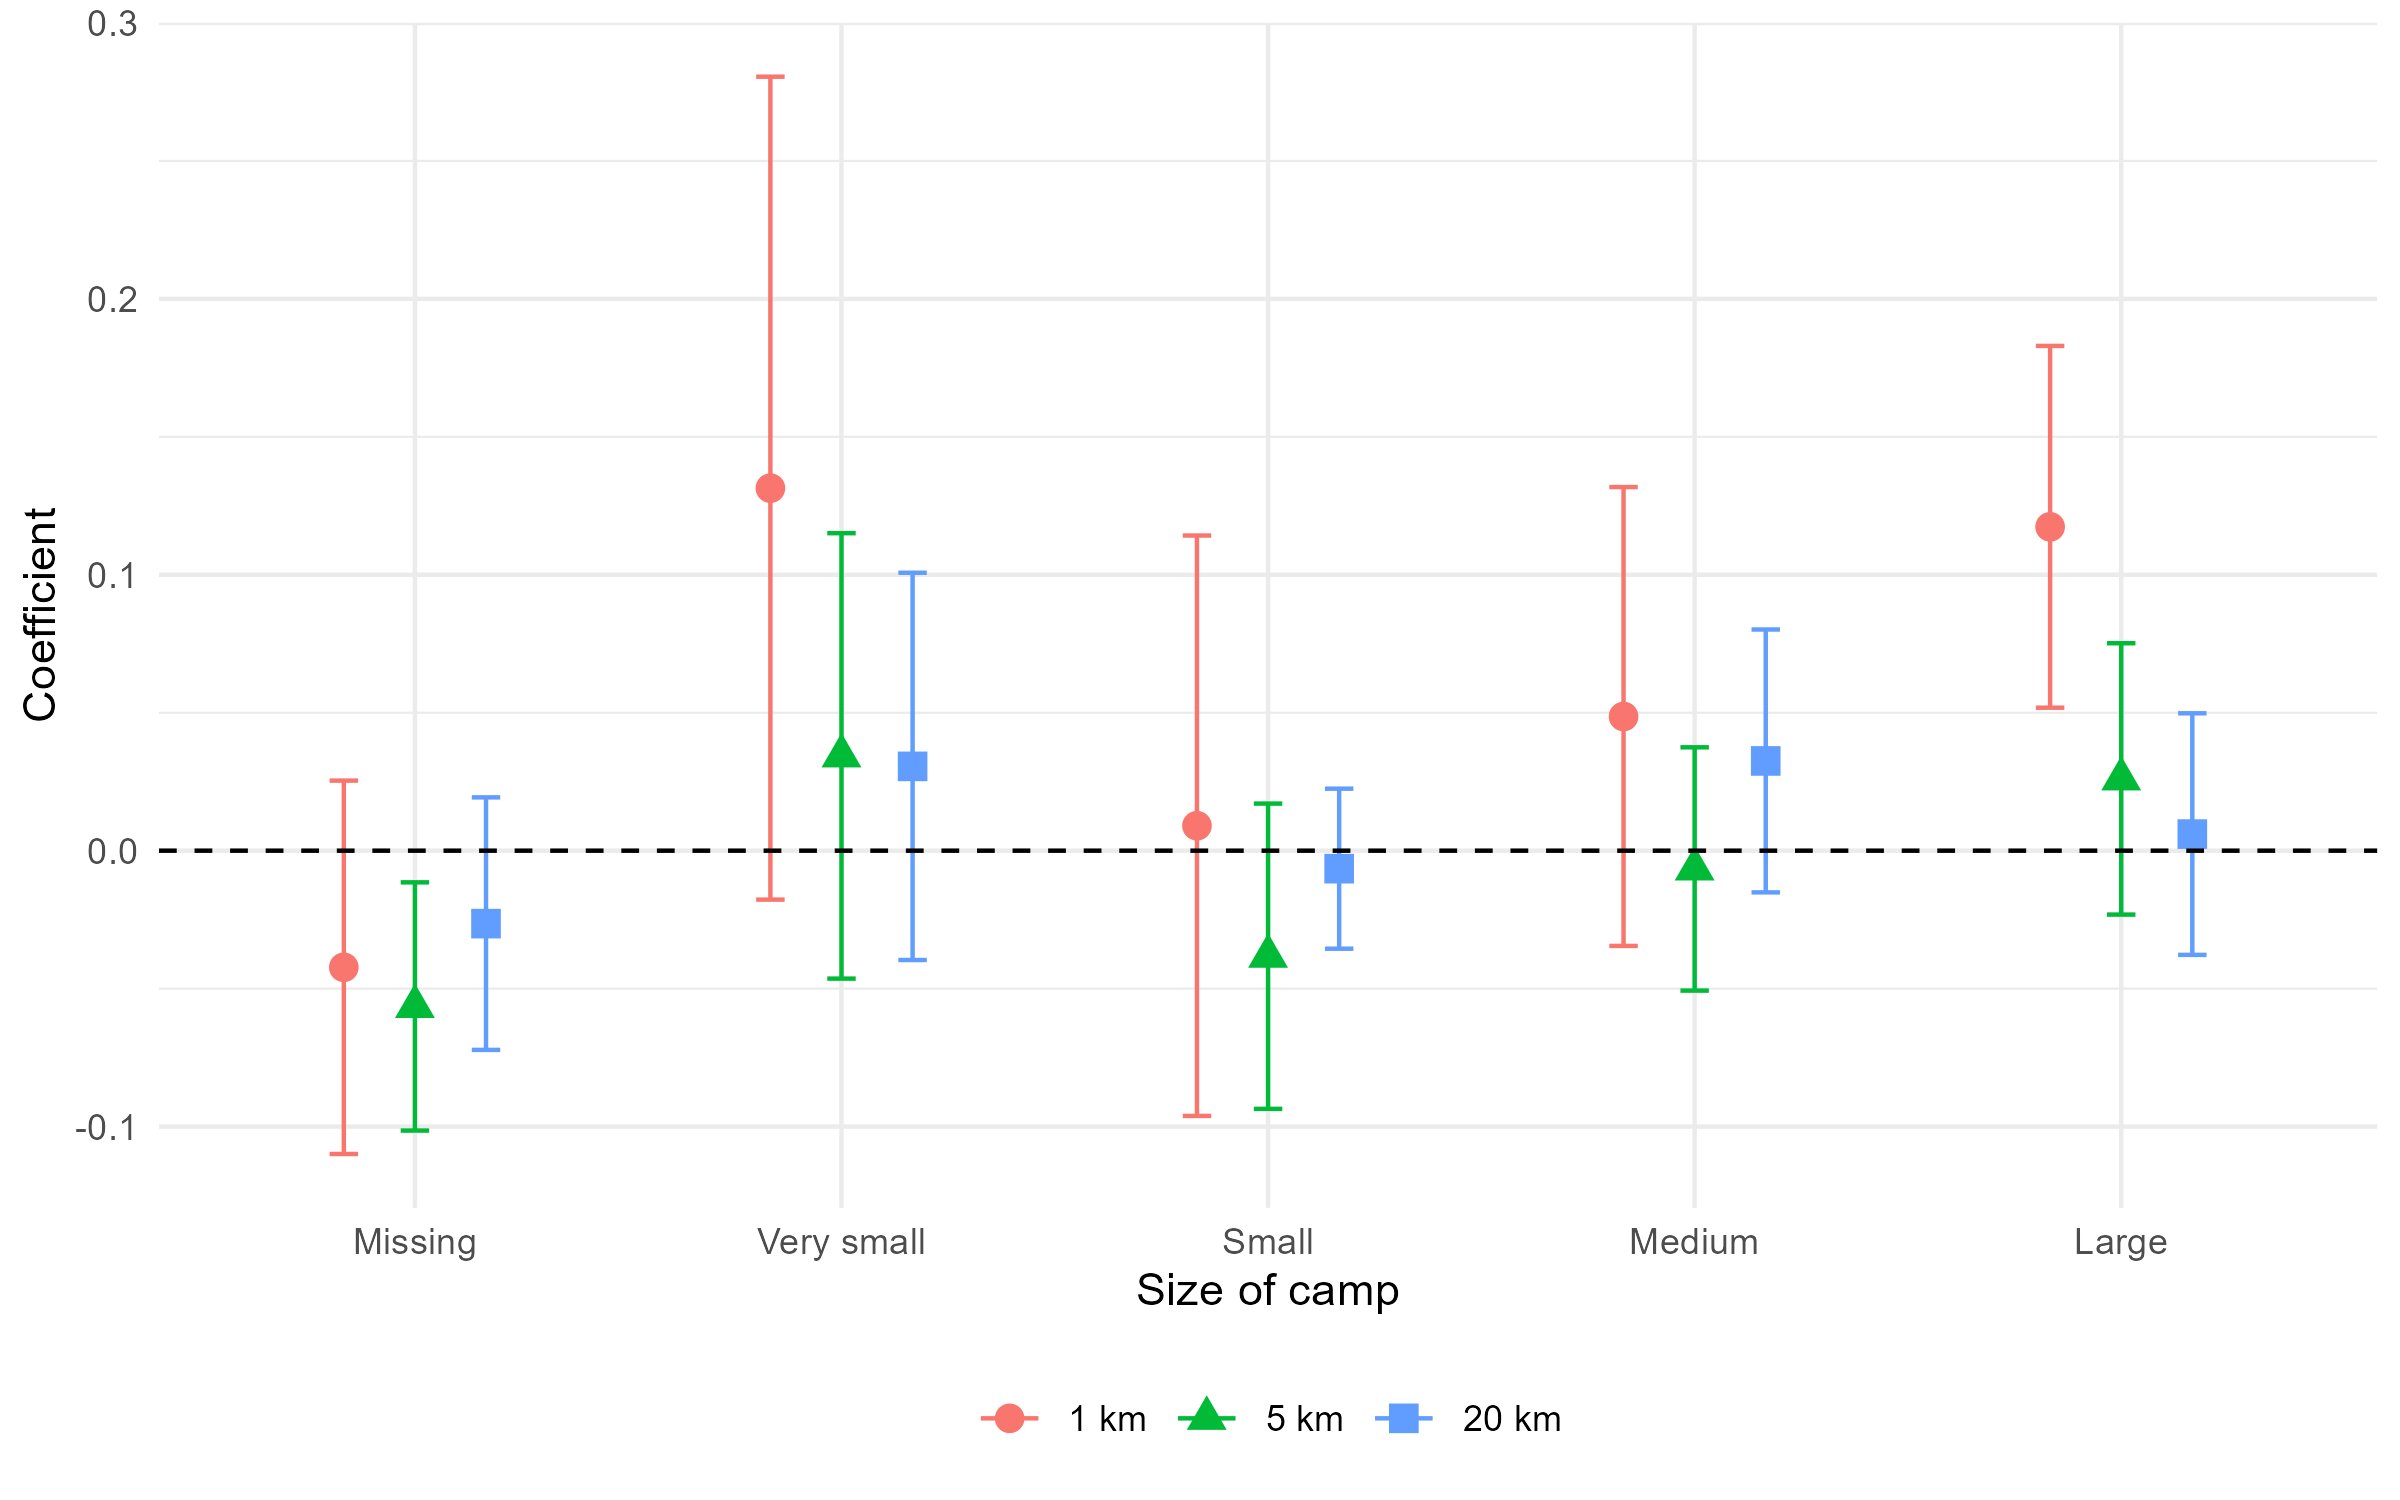
\includegraphics[width=0.8\linewidth]{figures/results/mobilisation/by_size_resistants.png}
  \label{fig:resistants}
   \begin{minipage}{0.8\textwidth}
        \vspace{0.1in} 
        {\footnotesize Notes: This graph reports the estimates of Poisson regressions on the number of resistants against Nazi Occupation. Error bars plot the interval confidence at 95\%. Standard errors are clustered to account for spatial correlation using \citet{conley_gmm_1999} (100 km). All specifications include region fixed effects and a set of controls—surname-based birthplace composition, altitude, mining activity, buildings per capita, average rainfall and the share of votes for the political parties of the 1936 legislative elections —and include a population offset.\par}
        \end{minipage}
\end{figure}


We further explore the political mobilization impact of exposure to Spanish refugees by examining its effect on the creation of associations. To assess this, we classify associations based on their names and descriptions of activities as listed in the Registre National des Associations. Our main results regarding these outcomes are presented in \autoref{tab:att_associations_large_medium}\footnote{The corresponding event study plots are available in \autoref{apdx:}}. Specifically, we identify four types of associations of interest: associations related to Migrants and Refugees, Solidarity associations, Left-wing and Union associations, and those focused on military and Resistance activities\footnote{We determine whether an association belongs to one of these categories based on a list of key words that unequivocally indicate the type of activity. These lists of key words are available in the Appendix.}. We then apply the same empirical strategies as before at the canton level, comparing localities that have welcomed large and medium camps of refugees with those that have not. Our findings show a positive effect on the creation of associations after the Retirada for associations related to refugee support, as well as for unions and left-wing groups. As a placebo, we also demonstrate that other types of associations, such as sports and religious groups, do not exhibit the same effects (see columns (5) and (6), showing results for these types of associations). While this effect aligns with the political mobilization observed through voting patterns post-WWII, as well as the backlash against the Socialist Party and the Radicals, our results also provide evidence of the type of interactions that may have contributed to the rise in both Resistance behaviour and the transmission of values.



\begin{table}[h!]
    \centering
    \caption{Association Creations, by Type, pre- and post- WWII}
    \resizebox{\textwidth}{!}{
\begingroup
\centering
\begin{tabular}{lcccccc}
   \toprule
                                     & Refugees      & Solidarity    & Unions/Left-wing & Resistance     & Sport         & Religion\\  
                                     & (1)           & (2)           & (3)              & (4)            & (5)           & (6)\\  
   \midrule 
   Large/Medium $\times$ civil war   & 0.5597        & 0.1689        & 0.1660$^{**}$    & -0.0010        & 0.0825        & -0.0093\\   
                                     & (0.4194)      & (0.1915)      & (0.0751)         & (0.0954)       & (0.0551)      & (0.2184)\\   
   Large/Medium $\times$ 1939     & 0.2568        & -0.3469       & 0.0579           & 0.1021         & 0.0289        & 0.2077\\   
                                     & (0.7100)      & (0.2655)      & (0.1417)         & (0.1712)       & (0.0972)      & (0.3350)\\   
   Large/Medium $\times$ 1940        & 1.489$^{**}$  & 0.5578        & 0.5441$^{**}$    & 0.7235$^{***}$ & 0.0290        & 0.2425\\   
                                     & (0.6344)      & (0.3633)      & (0.2116)         & (0.1940)       & (0.1778)      & (0.4230)\\   
   Large/Medium $\times$ 1944        & 1.035         & 0.7301        & 0.7710$^{***}$   & 0.0907         & 0.0196        & -0.3063\\   
                                     & (0.6546)      & (0.4610)      & (0.2701)         & (0.2330)       & (0.1506)      & (0.4596)\\   
   Large/Medium $\times$ 1945        & 1.266$^{**}$  & 0.0219        & 0.0799           & 0.3513$^{***}$ & 0.0144        & 0.0247\\   
                                     & (0.5680)      & (0.2097)      & (0.1947)         & (0.1144)       & (0.0707)      & (0.2454)\\   
   Large/Medium $\times$ 1946        & 0.9083        & 0.2943        & 0.1716           & 0.1340         & 0.0606        & -0.3760\\   
                                     & (0.6377)      & (0.2263)      & (0.1096)         & (0.1285)       & (0.0722)      & (0.2859)\\   
   Large/Medium $\times$ 1947-1950   & 0.9719$^{**}$ & 0.2175        & -0.0698          & 0.0864         & 0.0209        & 0.0600\\   
                                     & (0.4870)      & (0.1694)      & (0.0771)         & (0.1057)       & (0.0537)      & (0.1773)\\   
   Controls                          & $\checkmark$  & $\checkmark$  & $\checkmark$     & $\checkmark$   & $\checkmark$  & $\checkmark$\\   
    \\
   Observations                      & 1,946         & 10,067        & 23,622           & 20,738         & 29,564        & 9,156\\  
   Squared Correlation               & 0.70419       & 0.71786       & 0.76483          & 0.74927        & 0.85439       & 0.67070\\  
   Pseudo R$^2$                      & 0.32031       & 0.35288       & 0.41897          & 0.37466        & 0.46583       & 0.34794\\  
   BIC                               & 9,323.1       & 37,367.1      & 82,164.3         & 70,691.1       & 119,750.8     & 34,014.4\\  
    \\
   canton fixed effects              & $\checkmark$  & $\checkmark$  & $\checkmark$     & $\checkmark$   & $\checkmark$  & $\checkmark$\\   
   arrondissement-year fixed effects & $\checkmark$  & $\checkmark$  & $\checkmark$     & $\checkmark$   & $\checkmark$  & $\checkmark$\\   
   \bottomrule
\end{tabular}
\par\endgroup


}
    \label{tab:att_associations_large_medium}
    \par
        \begin{minipage}{\textwidth}
        \vspace{0.5em}
            \footnotesize
            Note: The table above reports coefficient of the Poisson estimates difference-in-differences regression at the canton level, comparing canton that have welcomed refugees with the ones that have not. Here treatment is only taking into account medium-size and large-size camps. To ensure comparability, control only takes into account the canton that are within a buffer of 40 km around this types of camps. We control for the total population of the canton per year as well as for the left-wing last election results. Our main specification takes into account canton fixed effects and arrondissement $\times$ year fixed effect. *** p$<$0.01, ** p$<$0.05, * p$<$0.1.
        \end{minipage}
\end{table}

%\clearpage
%\section{Mechanisms}\label{sec:mechanisms}
%

\subsection{Type of Backlash}



\subsection{Persistence}


We examine whether the location of refugee camps predicts where Spanish refugees ultimately settled after the Second World War, using data covering the universe of asylum applicants after 1945—approximately 160,000 individuals. Table~4 documents a strong and robust relationship between the presence of a refugee camp and subsequent refugee settlement. Across alternative functional forms, the coefficient on Camp remains positive and statistically significant. These results indicate that camps did not merely generate short-lived exposure to displaced populations but translated into persistent local settlement. This supports a demographic channel whereby refugee camps altered the composition of the local population, partially explaining the persistence of the political effects. As shown in \Cref{fig:refugees}, it also explains spillovers into control municipalities, as the relationship decreases with distance to the camp but remains statistically significant.

\begin{table}
\centering
\caption{Relationship between the refugees and the camps}
\centering
\begin{tabular}[t]{lcccc}
\toprule
  & (1) & (2) & (3) & (4)\\
\midrule
Within 1 km & 11.487 & 0.627*** & 0.422*** & 0.753***\\
\bottomrule
\multicolumn{5}{l}{\rule{0pt}{1em}* p $<$ 0.05, ** p $<$ 0.01, *** p $<$ 0.001}\\
\multicolumn{5}{l}{\rule{0pt}{1em}Column (1): OLS with fixed effects; column (2): ln.}\\
\multicolumn{5}{l}{\rule{0pt}{1em}Column (3): Poisson regression. Column (4): IHS / asinh}\\
\end{tabular}
\end{table}


\begin{table}
\centering
\caption{Characteristics of the refugees}
\centering
\begin{tabular}[t]{lcccccc}
\toprule
  & Left & No-left & High-skilled & Low-skilled & Nat & No Nat\\
\midrule
Camp & 0.390*** & 0.657*** & 0.486*** & 0.528*** & 0.314*** & 0.638***\\
\bottomrule
\multicolumn{7}{l}{\rule{0pt}{1em}* p $<$ 0.05, ** p $<$ 0.01, *** p $<$ 0.001}\\
\end{tabular}
\end{table}


\begin{figure}[htbp]
  \centering
  \caption{Relationship between refugee camps and refugees}
  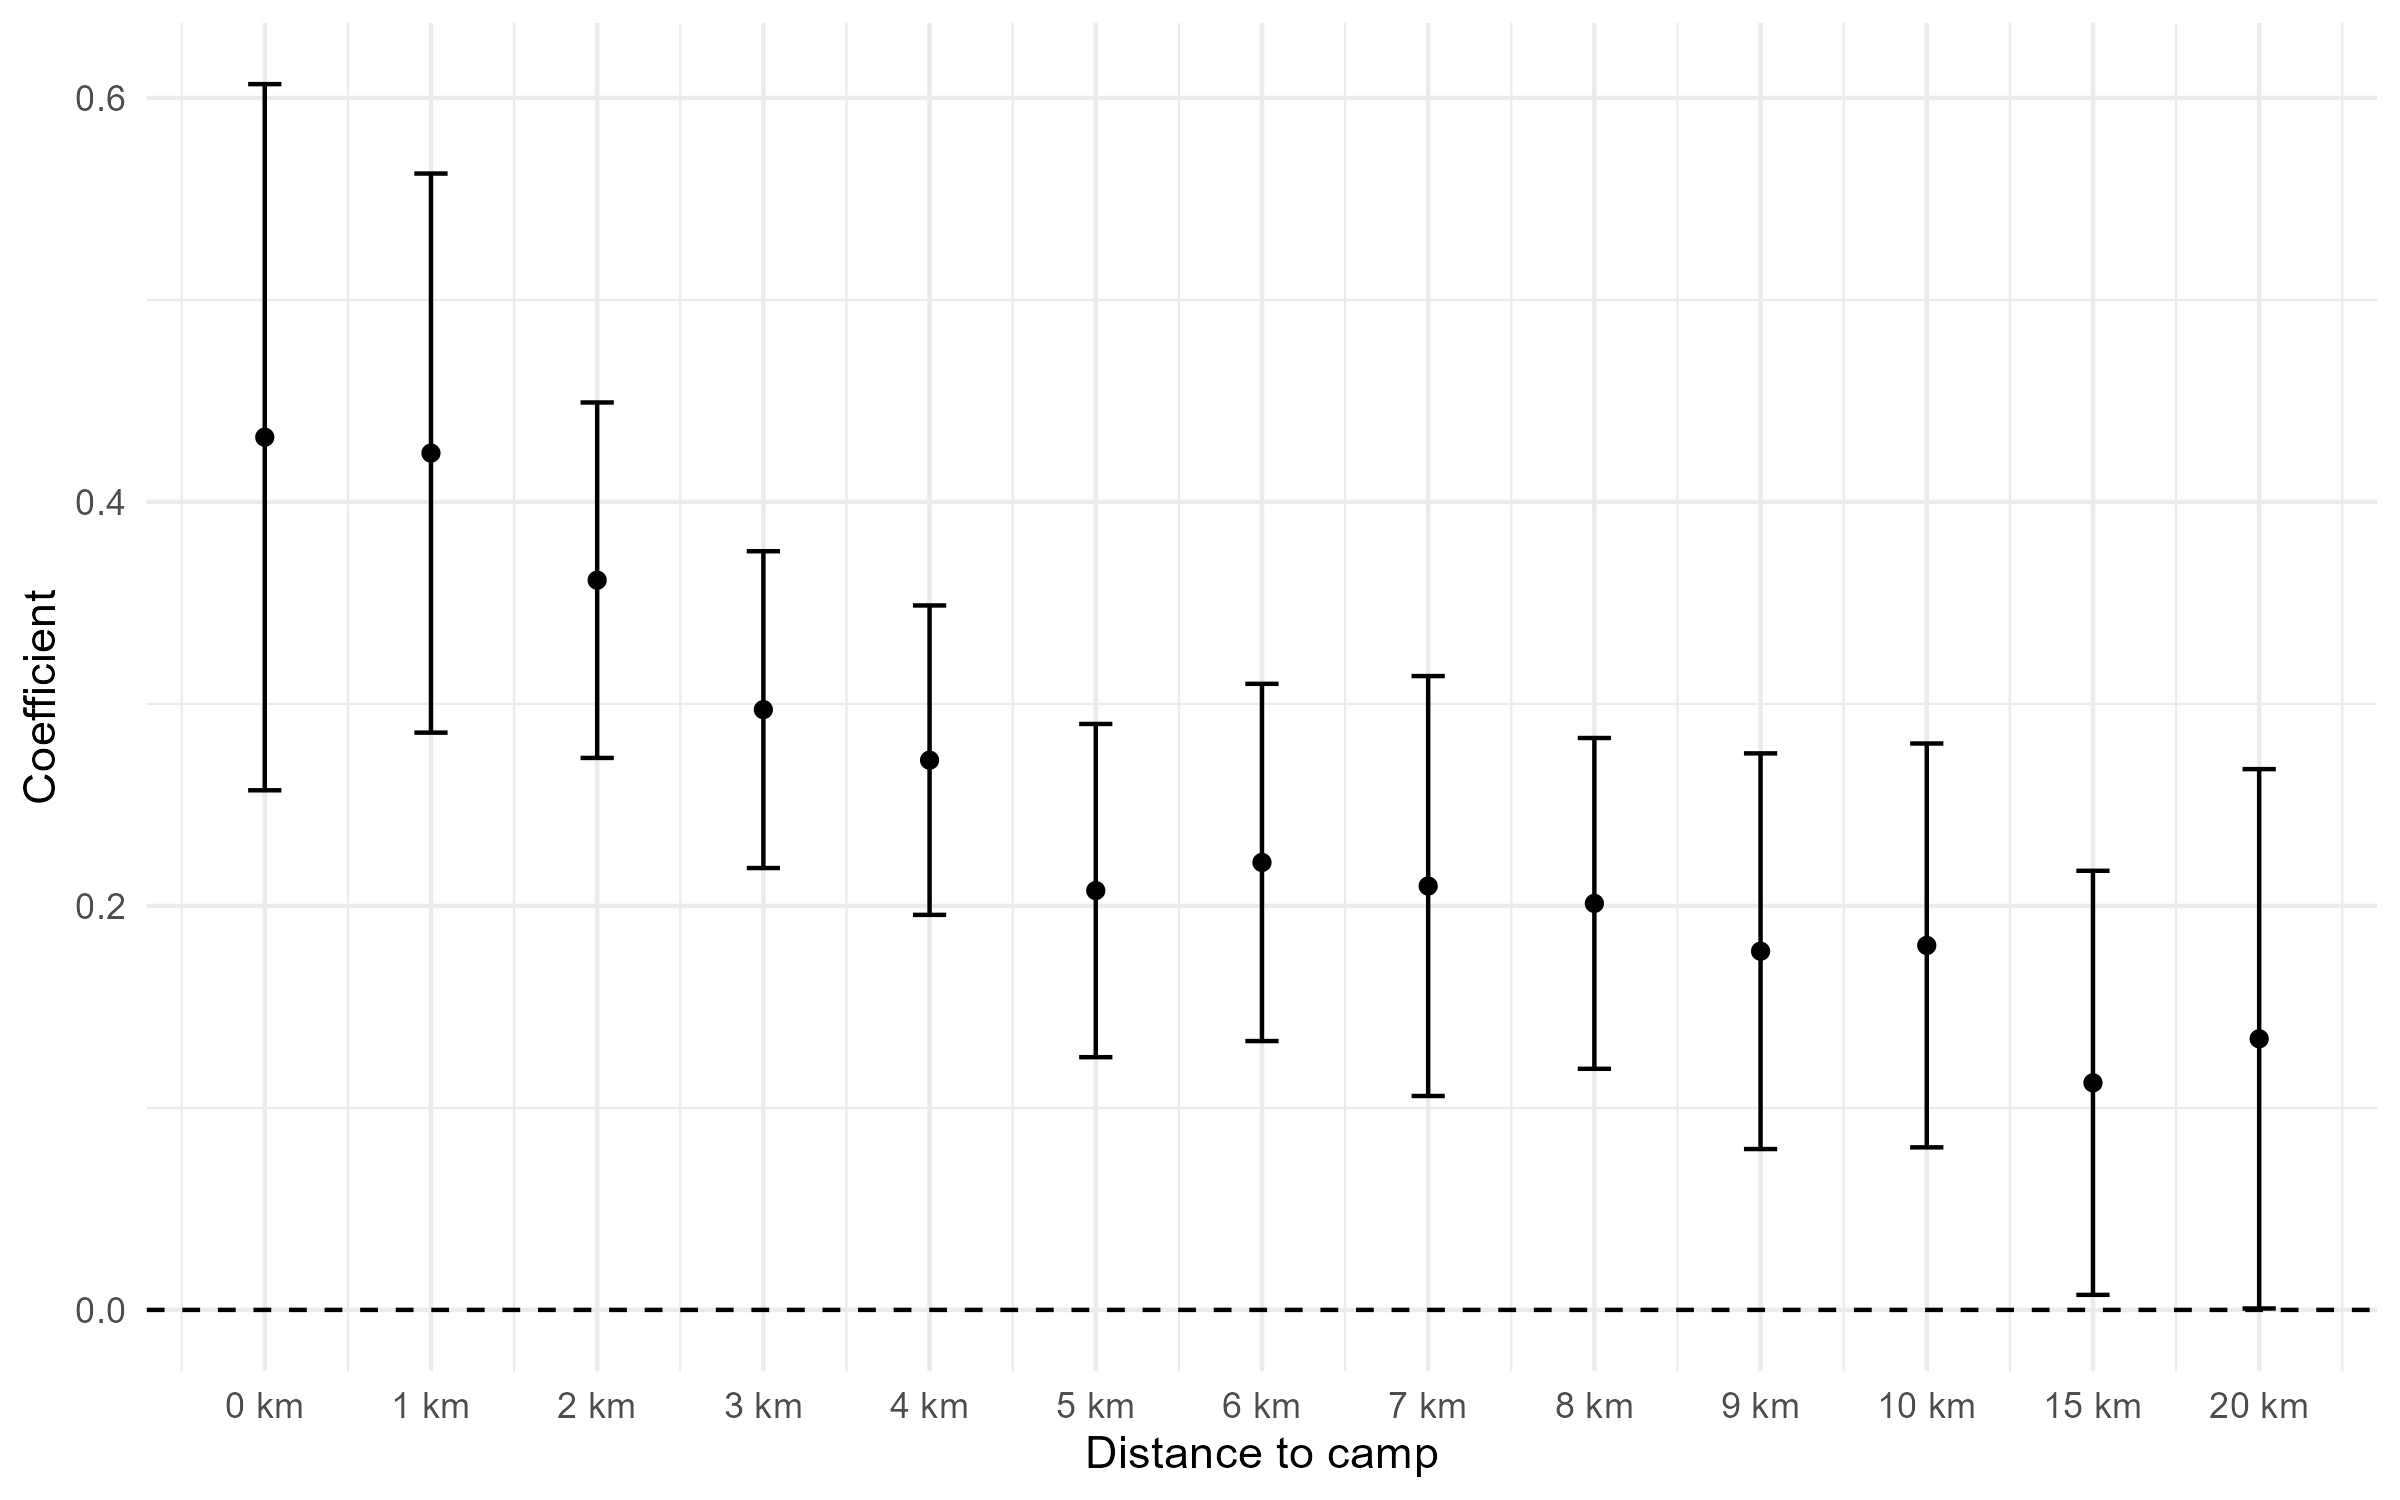
\includegraphics[width=0.8\linewidth]{figures/mechanisms/refugees_poisson.png}
  \label{fig:refugees}
   \begin{minipage}{0.7\textwidth}
        \vspace{0.5em}
        {\footnotesize Notes: This graph reports the estimates of Poisson regressions on the number of refugees after 1945. Standard errors are clustered to account for spatial correlation using \citet{conley_gmm_1999} (100 km). All specifications include department fixed effects and a set of controls—surname-based birthplace composition, altitude, mining activity, buildings per capita, average rainfall and the share of votes for the political parties of the 1936 legislative elections —and include a population offset.\par}
        \end{minipage}
\end{figure}




The results cannot be attributed to the electoral behaviour of the Spanish Republican refugees themselves. Legislative suffrage was restricted to French nationals, and the Vichy regime had dismantled the pre-war naturalization regime. Following the Liberation, the Ordinance of 19 October 1945 imposed a five-year residence requirement for naturalization, with eligibility additionally granted upon reaching majority after residing in France since age sixteen, or through marriage to a French national—although only 15\% of Spanish marriages between 1945 and 1950 were mixed \citep{Angoustures1997}. Code of 19 October 1945 also waived the residency requirement for volunteer enlistees, veterans of the two wars and members of the Resistance. Considering this framework, merely 6,400 Spaniards acquired the French nationality in 1946 \citep{spire_thave_1999}. Until 1978, slightly more than 15000 of Spanish refugees registered with the French Office for the Protection of Refugees acquired French nationality \citep{siglo_inmigracion_2009}. Moreover, newly naturalized individuals remained subject to legal incapacities: they were excluded from the electoral rolls for five years after naturalization and barred from holding elected office for ten years \citep{code_nationalite_fr_1945}. For these reasons, the settlement of Spanish refugees could not have mechanically translated into direct electoral participation.

\section{Robustness}\label{sec:robustness}







We discuss in this section the robustness of our results.\\
We first show that the backlash phenomenon that we measure is consistent between French geographical regions. To do so, we re-estimate our preferred specification on a series of sub-samples in which we sequentially exclude each broad region from the analysis. We display these results in \autoref{fig:by_region}. Dropping the regions in the North of France, the estimated backlash effect becomes larger in magnitude. This is consistent with the fact that Northern camps were, on average, less visible, of a smaller size and generated fewer local tensions. It is also consistent with the difference in the composition of the hosted population: Northern camps and centres welcome a higher share of women and children, which plausibly reduces the magnitude of the backlash effect we measure. Consistently, when we exclude regions in the South, the estimated coefficient moves towards zero and the implied backlash is smaller, in line with the idea that camps in the South were more visible and politically salient. The pattern of our results is nevertheless preserved across all leave-one-out specifications: the sign of the estimated effect remains unchanged. Overall, this suggests that no single region is driving our main results.

\begin{figure}[htbp]
  \centering
  \caption{Effect on socialist vote share - Leave one out results}
  
\includegraphics[width=0.6\linewidth]{../figures/results/political/by_region_sfio.png}
  \label{fig:by_region}
   \begin{minipage}{0.7\textwidth}
   \vspace{0.1in} 
        {\tiny Notes: This graph reports the estimates leaving one region out at the time of the baseline TWFE. Error bars plot the interval confidence at 95\%. Standard errors are clustered at the municipal level.\par}
        \end{minipage}
\end{figure}

\begin{figure}[htbp]
  \centering
  \caption{Effect on communist vote share - Leave one out results}
  
\includegraphics[width=0.6\linewidth]{../figures/results/political/by_region_pcf.png}
  \label{fig:by_region}
   \begin{minipage}{0.7\textwidth}
   \vspace{0.1in} 
        {\tiny Notes: This graph reports the estimates leaving one region out at the time of the baseline TWFE. Error bars plot the interval confidence at 95\%. Standard errors are clustered at the municipal level.\par}
        \end{minipage}
\end{figure}

Similarly, we verify that our results are not driven by differential dynamics between the part of the country occupied by the German forces (\textit{zone occupée}) and the municipalities under the authority of the Vichy government (\textit{zone libre}). Exploiting this historical division also allows us to use occupation status as a proxy for the local intensity of the Second World War and to check whether our estimates are simply capturing the areas most directly affected by the conflict.

In order to do so, we re-estimate our baseline specification separately for municipalities located in the occupied and in the non-occupied zones. \autoref{fig:occupied} shows the results. Trends between treated and control municipalities are similar when we restrict the sample to the occupied zone and when we restrict it to the non-occupied zone, indicating that our main findings are not specific to one side of the demarcation line. If anything, the estimated backlash is of a larger magnitude in the non-occupied areas, where the largest camps and soldiers refugee settlements are located. If the intensity of the war were driving our results, one would instead expect stronger effects in the occupied zone. This pattern reinforces the interpretation that our estimates capture a backlash mechanism linked to the presence of the camps rather than to wartime violence.

\begin{figure}[htbp]
  \centering
  \caption{Effect on socialist vote share - Occupied vs Non-Occupied areas}
  
\includegraphics[width=0.7\linewidth]{../figures/results/political/occupied_sfio.png}
  \label{fig:occupied}
    \begin{minipage}{0.7\textwidth}
   \vspace{0.1in} 
   {\tiny Notes: This figure reports difference-in-differences estimates separately for the Nazi-occupied zone and the non-occupied Vichy zone. Error bars show 95\% confidence intervals. Standard errors are clustered at the municipality level.\par}
        \end{minipage}
\end{figure}

\begin{figure}[htbp]
  \centering
  \caption{Effect on communist vote share - Occupied vs Non-Occupied areas}
  
\includegraphics[width=0.7\linewidth]{../figures/results/political/occupied_pcf.png}
  \label{fig:occupied}
    \begin{minipage}{0.7\textwidth}
   \vspace{0.1in} 
   {\tiny Notes: This figure reports difference-in-differences estimates separately for the Nazi-occupied zone and the non-occupied Vichy zone. Error bars show 95\% confidence intervals. Standard errors are clustered at the municipality level.\par}
        \end{minipage}
\end{figure}

SYNTHETIC DID 

\begin{table}[h!]
    \centering
    \caption{Impact of refugee camp exposure on the vote shares - Synthetic DiD}
    \resizebox{0.4\textwidth}{!}{\begin{tabular}{lcccc}
\toprule
 & \multicolumn{2}{c}{\textit{SFIO Vote Share}} & \multicolumn{2}{c}{\textit{PCF Vote Share}} \\
\cmidrule(lr){2-3}\cmidrule(lr){4-5}
 & (1) SDID & (2) SDID + Cov. & (1) SDID & (2) SDID + Cov. \\
\midrule
Within 1 km & -0.0328*** & -0.0314*** & 0.0287*** & 0.0285*** \\
 & (0.0033) & (0.0066) & (0.0037) & (0.0023) \\
Ring 5--10 km & -0.0232*** & -0.0232*** & 0.0289*** & 0.0287*** \\
 & (0.0024) & (0.0019) & (0.0041) & (0.0023) \\
Ring 10--15 km & -0.0205** & -0.0206*** & 0.0197*** & 0.0194*** \\
 & (0.0096) & (0.0033) & (0.0049) & (0.0013) \\
Ring 15--20 km & -0.0176*** & -0.0177*** & 0.0149*** & 0.0148*** \\
 & (0.0022) & (0.0007) & (0.0020) & (0.0017) \\
Ring 20--25 km & -0.0118*** & -0.0118*** & 0.0086*** & 0.0083*** \\
 & (0.0033) & (0.0015) & (0.0013) & (0.0025) \\
Ring 30--35 km & 0.0042 & 0.0047 & -0.0019 & -0.0022 \\
 & (0.0039) & (0.0029) & (0.0024) & (0.0018) \\
\bottomrule
\multicolumn{5}{l}{\footnotesize Standard errors in parentheses. $^{*}p<0.10$, $^{**}p<0.05$, $^{***}p<0.01$} \\
\end{tabular}
}
    \label{table:table_synthetic}
    \par
        \begin{minipage}{0.4\textwidth}
        \vspace{0.5em}
            \footnotesize
            Note: The table reports the synthetic DiD estimates of being located within a given distance ring from the refugee camps. The control group are those within 20-40km.  Standard errors (SE) are obtained using the placebo procedure. *** p$<$0.01, ** p$<$0.05, * p$<$0.1.
        \end{minipage}
\end{table}

\begin{figure}[htbp]
  \centering
  \caption{Effect on socialist vote share - Comparative between DiD and synthetic DiD}
  
\includegraphics[width=0.7\linewidth]{../figures/results/political/comparison_sfio.png}
  \label{fig:comparison}
    \begin{minipage}{0.7\textwidth}
   \vspace{0.1in} 
   {\tiny Notes: .\par}
        \end{minipage}
\end{figure}


\begin{figure}[htbp]
  \centering
  \caption{Effect on communist vote share - Comparative between DiD and synthetic DiD}
  
\includegraphics[width=0.7\linewidth]{../figures/results/political/comparison_pcf.png}
  \label{fig:comparison}
    \begin{minipage}{0.7\textwidth}
   \vspace{0.1in} 
   {\tiny Notes: .\par}
        \end{minipage}
\end{figure}


\begin{figure}[htbp]
  \centering
  \caption{Effect on socialist vote share - Synthetic event study}
  
\includegraphics[width=0.7\linewidth]{../figures/results/political/sdid_event_SFIO.png}
  \label{fig:comparison}
    \begin{minipage}{0.7\textwidth}
   \vspace{0.1in} 
   {\tiny Notes: .\par}
        \end{minipage}
\end{figure}

\begin{figure}[htbp]
  \centering
  \caption{Effect on communist vote share - Synthetic event study}
  \includegraphics[width=0.7\linewidth]{../figures/results/political/sdid_event_PCF_pop.png}
  \label{fig:comparison}
    \begin{minipage}{0.7\textwidth}
   \vspace{0.1in} 
   {\tiny Notes: .\par}
        \end{minipage}
\end{figure}


CONTINUOUS DID 

The table is significant 
%\begin{table}[h!]
\centering
\caption{Impact of Camps and Refugees on Vote Shares (TWFE)}
\label{tab:twfe_camps_refugees}
\begin{tabular}{lcccc}
\hline
 & \multicolumn{2}{c}{SFIO vote share} & \multicolumn{2}{c}{PCF vote share} \\
 & (1) Camps & (2) Refugees & (3) Camps & (4) Refugees \\
\hline

Post $\times$ Camps (1 km) 
& -0.0159*** &  & 0.0115*** &  \\
 & (0.00347) &  & (0.00323) &  \\

Post $\times$ Refugees (1 km) 
&  & -3.20e-06** &  & 3.97e-07 \\
 &  & (1.11e-06) &  & (1.01e-06) \\

\hline
Observations & 74,781 & 74,781 & 74,781 & 74,781 \\
Municipality FE & Yes & Yes & Yes & Yes \\
Year $\times$ Arrondissement FE & Yes & Yes & Yes & Yes \\
\hline
\multicolumn{5}{l}{\footnotesize Standard errors clustered at the municipality level in parentheses.} \\
\multicolumn{5}{l}{\footnotesize *** $p<0.01$, ** $p<0.05$, * $p<0.1$.}
\end{tabular}
\end{table} % file not yet available

\begin{figure}[htbp]
  \centering
  \caption{Effect on socialist vote share - Continous DiD}
  
\includegraphics[width=0.7\linewidth]{../figures/results/political/cont_es_sfio_camps.png}
  \label{fig:comparison}
    \begin{minipage}{0.7\textwidth}
   \vspace{0.1in} 
   {\tiny Notes: .\par}
        \end{minipage}
\end{figure}

\begin{figure}[htbp]
  \centering
  \caption{Effect on communist vote share - Continous DiD}
  
\includegraphics[width=0.7\linewidth]{../figures/results/political/cont_es_pcf_camps.png}
  \label{fig:comparison}
    \begin{minipage}{0.7\textwidth}
   \vspace{0.1in} 
   {\tiny Notes: .\par}
        \end{minipage}
\end{figure}


\newpage
\section{Conclusion}\label{sec:conclusion}
This paper examines the long-term political effects of the 1939 mass displacement of Spanish Republican refugees into France, leveraging the quasi-random geography of internment camp placement as a natural experiment. Using geocoded data on refugee camps and detailed municipal-level electoral and resistance records, we assess how proximity to refugee camps shaped political behaviour during and after World War II.

We find that exposure to refugee camps is associated with a persistent decrease in support for the socialist SFIO party, suggesting a lasting political backlash in host communities. At the same time, proximity to camps increases both Communist Party vote shares and local participation in resistance activities, indicating that refugee presence also facilitated the diffusion of political ideas and collective mobilization. These findings confirm that refugee influence is dual: it can act as a source of perceived political threat for some segments of the host population, while serving as a vector of ideological transmission and mobilisation for others.

By isolating plausibly exogenous variation in refugee settlement, our study contributes to a growing literature on the political legacy of forced migration and the transmission of political preferences. Unlike most work that focuses on recent or voluntary migration, our setting involves culturally proximate but politically selected refugees, allowing us to disentangle competing mechanisms of backlash and diffusion. We also complement research showing that contact conditions matter: short-term, coercive exposure can exacerbate fears, whereas more sustained interaction may facilitate norm transmission and political engagement. The heterogeneity we document aligns with the idea that forced displacement can generate political polarization.

Overall, our findings underscore the relevance of historical refugee episodes for understanding persistent political polarization and the long-run consequences of displacement on host communities. They also offer broader insights into the political economy of refugee reception, especially in contexts where administrative capacity is limited and resettlement policies are improvised.








%%%%%%%%%%%%%%%%%%%%%%%%%%%%%%%%%%%%%%%%%%%%%%%%%
\clearpage
\begin{singlespace}
%\bibliographystyle{plainnat}
\bibliographystyle{chicago}
\bibliographystyle{aer}
\bibliography{bibliography}
\end{singlespace}
%%%%%%%%%%%%%%%%%%%%%%%%%%%%%%%%%%%%%%%%%%%%%%%%%

\clearpage
\appendix


\section*{Appendix}\label{sec:appendix}

\section{Additional Tables and Figures}

\Cref{fig:map_example_methodology} plots how the buffers are defined using as an example the department of Gers. The darker areas represent municipalities located within 1 km of a camp, while the lighter areas correspond to those between 1 km and 5 km. 

\begin{figure}[htbp]
  \centering
  \caption{Refugee Camps and Exposure Buffers}
  
\includegraphics[width=0.6\linewidth]{../figures/map_example_methodology.png}
  \label{fig:map_example_methodology}
   \begin{minipage}{0.7\textwidth}
   \vspace{0.1in} 
        {\tiny Notes: This map show how we define buffers around the locations of refugees camps. The example show it the \textit{département} of Gers (32) in the region Occitanie. The municipalities that appear in light green are the ones for which part of the territory falls in the 5 kilometres buffers, drawn in dashed line. \par}
        \end{minipage}
\end{figure}



\begin{figure}[htbp]
  \centering
  \caption{Distribution of Camps Sizes}
  
\includegraphics[width=0.8\linewidth]{../figures/bars_camps_sizes.png}
  \label{fig:bars_camps_sizes}
   \begin{minipage}{0.7\textwidth}
   \vspace{0.1in} 
        {\tiny Notes: This graph shows the distribution of camps, depending on the total population of refugees they welcome. The different colors represent the different categories we use in our analysis. They represent the four quartiles based on the reported population of the camps in our data (excluding camps for which the information is missing).   \par}
        \end{minipage}
\end{figure}



\begin{table}[h!]
    \centering
    \caption{Impact of refugee camps on right-wing support}
    \resizebox{0.6\textwidth}{!}{\begingroup
\centering
\begin{tabular}{lcc}
   \toprule
                                 & Spillovers     & Control as 20-40km \\   
                                 & (1)            & (2)\\  
   \midrule 
   Within 1 km                   & 0.0074$^{*}$   & 0.0121$^{*}$\\   
                                 & (0.0042)       & (0.0064)\\   
   Ring 5                        & -0.0023        &   \\   
                                 & (0.0036)       &   \\   
   Ring 10                       & -0.0037        &   \\   
                                 & (0.0035)       &   \\   
   Ring 15                       & -0.0067$^{**}$ &   \\   
                                 & (0.0034)       &   \\   
   Ring 20                       & -0.0014        &   \\   
                                 & (0.0034)       &   \\   
   Ring 25                       & -0.0053        &   \\   
                                 & (0.0035)       &   \\   
   Ring 30                       & -0.0057        &   \\   
                                 & (0.0036)       &   \\   
    \\
   R$^2$                         & 0.801          & 0.824\\  
   Observations                  & 261,959        & 74,926\\  
    \\
   Municipality fixed effects & $\checkmark$   & $\checkmark$\\   
   Time-Reg fixed effects     & $\checkmark$   & $\checkmark$\\   
   \bottomrule
\end{tabular}
\par\endgroup
}
    \label{table:right_results}
        \vspace{0.5em}
        \begin{minipage}{0.6\textwidth}
            \footnotesize
            Note: In the first column, we estimate the two-way fixed effects, restricting the control group to those within 20km. In the second column, the control group are those within 10km. In the third column, we estimate \cref{equation:political}. Standard errors (SE) are clustered at the municipality level. *** p$<$0.01, ** p$<$0.05, * p$<$0.1.
        \end{minipage}
\end{table}


\begin{figure}[htbp]
  \centering
  \caption{Impact of refugee camps on socialist vote share - ring estimations}
  
\includegraphics[width=0.8\linewidth]{../figures/results/political/pvoixSFIO_event_study.png}
  \label{fig:SFIO_all}
   \begin{minipage}{0.7\textwidth}
        \vspace{0.5em}
        {\footnotesize Notes: This graph reports the estimates from \cref{equation:political}, where the coefficient for each ring is estimated using municipalities located 20–40 km away as the control group. Error bars plot the interval confidence at 95\%. Standard errors are clustered at the municipality level.\par}
        \end{minipage}
\end{figure}


\begin{figure}[htbp]
  \centering
  \caption{Impact of refugee camps on communist vote shares - ring estimations}
  
\includegraphics[width=0.8\linewidth]{../figures/results/political/pvoixPCF_event_study.png}
  \label{fig:PCF_all}
   \begin{minipage}{0.7\textwidth}
        \vspace{0.5em}
        {\footnotesize Notes: This graph reports the estimates from \cref{equation:political}, where the coefficient for each ring is estimated using municipalities located 20–40 km away as the control group. Error bars plot the interval confidence at 95\%. Standard errors are clustered at the municipality level.\par}
        \end{minipage}
\end{figure}

\begin{figure}[htbp]
  \centering
  \caption{Impact of refugee camps on the socialist vote share - by size}
  
\includegraphics[width=0.8\linewidth]{../figures/results/political/sfio_size.png}
  \label{fig:SFIO_all}
   \begin{minipage}{0.7\textwidth}
        \vspace{0.5em}
        {\footnotesize Notes: This graph reports the estimated effect for each camp size, using as the control group municipalities without any other type of camp located 20–40 km away. Error bars plot the interval confidence at 95\%. Standard errors are clustered at the municipality level.\par}
        \end{minipage}
\end{figure}

\begin{figure}[htbp]
  \centering
  \caption{Impact of refugee camps on the communist vote share - by size}
  
\includegraphics[width=0.8\linewidth]{../figures/results/political/communist_size.png}
  \label{fig:SFIO_all}
   \begin{minipage}{0.7\textwidth}
        \vspace{0.5em}
        {\footnotesize Notes: This graph reports the estimated effect for each camp size, using as the control group municipalities without any other type of camp located 20–40 km away. Error bars plot the interval confidence at 95\%. Standard errors are clustered at the municipality level.\par}
        \end{minipage}
\end{figure}

\begin{comment}

\clearpage
\section{Historical Context}


\subsection{The Arrival and Welcoming of the Refugees}

\subsubsection*{The Spanish Civil War and the Different Migrations Flows}

The large majority of the migrations flows from Spain, related with the Civil War, occur between 1936 and 1939. The timing of the migrations is directly related with the victories of the Nationalist groups over the Republicans. Dreyfus-Armand (2002) identifies three major waves of Spanish refugees to France between 1936 and 1939.
\begin{enumerate}
    \item The first one occurs in August 1936 and corresponds to the fall of the Republican force in the Basque Country. This wave is mainly composed of civilians, although soldiers also entered in French territory, mainly in order to reach Perpignan and then the Republican zone in Catalonia. Most of the refugees at this time are encouraged to come back to Spain. This wave represents around 15,000 refugees.
    \item The second wave occurs in 1937. The violence of the fighting between Republican and the Nationalists, especially the final assault against Bilbao, led the Republican authorities to evacuate the city. With the collaboration of the French authorities, more than 120,000 individuals, both soldiers and civilians.
    \item The last and biggest flow of refugees occurs in January 1939. This flow is known as ``La Retirada" (\textit{The Retreat}) and occurs after the Fall of Barcelona. This flow is both composed of soldiers but also civilians fleeing the intensive bombings. Most of the refugees cross the border by the Pyrenees, for instance in Le Perthus. Estimations of this amount of persons who cross the border differ. In March 1939, the French Assembly, through the Commission of Foreign Affairs, estimated that 450,000 refugees have crossed the border. At the same period, the French Ministry of Interior estimates that 300,000 soldiers and 214,000 civilians crossed the border. 
    \end{enumerate}

French Authorities, specially after 1938, initiate several policies in order to encourage the repatriation of refugees. For instance, at the end of 1938 and before the \textit{Retirada}, only 45,000 Spanish are still in France\footnote{from this number, a quarter are children according to J. Rubio, La Emigracion de la guerra civil de 1936-1939 (1982).}.

\subsubsection*{The Internment Camps}

Since the beginning of the Civil War, the guiding principle of the French Governments is to encourage repatriations of refugees. In a context of growing political tensions in Europe, the presence of thousands of refugees, some of who are politically very active, is considered as a major source of instability by the authorities. In Febuary 1939, France signed the Berard-Jordan Agreement with Franquist Spain, in order to facilitate the repatriation of refugees. As a consequence, between April 1rst 1939 (end of the Civil War) and the end of the year, thousands of refugees returned to Spain. During this time, the repatriation of refugees have been used several time by Franco to put pressure on the French Government, especially in order to push France to respect the terms of the agreement.
(for instance on the restitution of goods that had been transferred to France during the War). \\
In May-June 1939, evaluations estimates the number of refugees in France to be around 350,000 (including 155,000 civilians), and 250,000 in August of the same year\footnote{Archive du Ministère des Affaires Etrangères, série Europe 1918-1940), sous-série Espagne, vol. 189.}. At the end of 1939, French authorities estimated the number of refugees to be of 180,000 individuals (including 45,000 women and children)\footnote{Ibid.}. \\

The welcoming of refugees essentially considered as ``improvised", and refugees, both soldiers and families, are often put in old factories or closed down prison\footnote{Les camps sur la plage, un exil espagnol (avec Geneviève Dreyfus-Armand), Autrement, 1995}. Concentration camps are built for the first time in January 1939 when the largest amount of refugee starts to cross the border after the victories of Nationalists in Barcelona. 

\subsection{The Second World War and the Political Exile}

\subsubsection*{The Involvement during WWII}

\subsubsection*{The Post-War Exile until the Fall of Franco}

The exodus from Spain with the Civil War goes on after the Second World War and France Liberation. Estimations evaluate that around 10,000 immigrants from Spain have entered France each year between 1947 and 1949. 

\subsubsection*{The Political and Cultural Transmission}

\clearpage
\subsection{The Political Context in France}

\subsection*{Main parties during the interwar period}

The French Left during the interwar period was structured around three major political forces alongside several smaller organizations. The central pillars were the Radical-Socialists (RAD-SOC) —who, despite their name, occupied a space closer to liberal centrism—the Socialist Party (SFIO), and the Communist Party (PCF). Among the minor parties, the Republican Socialist Union held particular relevance, positioned ideologically between the Radicals and the Socialists, while a faction of dissident communists formed the Proletarian Union (Pickersgill, 1939)

In 1924, most of the left-wing parties (with the exception of the Communists) created an electoral alliance known as the Cartel des Gauches. This coalition achieved notable success in the legislative elections of 1924. Its cohesion weakened in 1928 and the the conservatives and moderates return to power under the leadership of Raymond Poincaré. The elections of 1932 once again give a majority to the Radicals and the Socialists. The Communists, however, remained outside of this arrangement until 1935, when the Third International urged communist parties across Europe to collaborate with democratic forces in the fight against fascism. This strategic shift laid the foundations of the Front Populaire, which brought together the full spectrum of left-wing parties (Pickersgill, 1939). Léon Blum, leader of the Socialist Party, becomes Prime Minister and his government implements a series of major social reforms as the introduction of the forty-hour work week \textcolor{red}{(Reference)}.

Following the classification of \cite{piketty_histoire_2023}, we divide the political forces present in the 1936 legislative elections in ten main forces. \textcolor{red}{(Reference)} for the explanation of the parties. 

\begin{description}
\item[Left-wing parties]: 
\begin{description}
    \item[PCF:] French Communist Party (Parti Communiste Français) and organizations close to the communists. Created in 1920 during the Tours Congress, when a majority of the SFIO decides to join the Third International (Comintern). At the time, it positions itself on the far left with a revolutionary and internationalist agenda. Its main leaders include Maurice Thorez and Jacques Duclos. 
    \item[SFIO:] Socialist party (Section Française de l’Internationale Ouvrière) and organizations close to the socialists. Created in 1905, it represents the Socialist movement. It adopts a Marxist orientation in theory but acts reformist in practice. Its most notable leaders are Léon Blum and Paul Faure.
    \item[RAD-SOC:] Candidates presented by the Radical Party (Parti Radical et Radical-Socialiste) and organizations close to the radicals. Founded iin 1901, the Radical and Radical-Socialist Party is France’s oldest political party. Influenced by Freemasonry, it championed civil liberties, anticlericalism, universal suffrage, and anti-colonialism. The party reached its peak in the interwar period under leaders like Édouard Herriot and Édouard Daladier. From the 1930s, while remaining anchored on the left (Cartel des gauches, Popular Front), it pursued moderate governance and came to embody “traditional” republican values—laïcité and free public education. During World War II, the party split between supporters of Pétain, resistance figures, and collaborators, suffering repression under Vichy. After Liberation, it was associated with the failed Third Republic and challenged by the MRP and SFIO. Attempts at modernization under Pierre Mendès France from 1955 exposed deep internal divisions, culminating in a right-wing split and the creation of the Centre républicain in 1956 francearchives_parti_radical \citep{francearchives_parti_radical}. 
    \item[DVG:] candidates presented by parties and organizations close to the communist or socialist movement (Proletarian Union, Communist Socialist Union, etc.).
    \item[USR:] candidates presented by the Republican Socialist Union and by related organizations (Independent Socialists, Independent Left, dissident Radical Party – Camille Pelletan, Young Republic, Frontist Party, etc.).

    \end{description}
\item[Right-wing parties]: 
\begin{description}
    \item[AD:] candidates presented by the Democratic Alliance and affiliated parties and organizations as Republican Left, Independent Radicals, Popular Democrats (Parti Démocrate Populaire), Independent Republicans, etc. Parti Démocrate Populaire (PDP) is founded in 1924, embodies Christian democratic and center-right values. One of its most important leaders is Auguste Champetier de Ribes. The PDP can be seen as the precursor to the postwar Mouvement Républicain Populaire (MRP).
    \item[FR-URD:] candidates presented by the Republican Federation (Fédération Républicaine) and the Republican and Democratic Union (as well as the National Republican Party). the Fédération Républicaine was founded in 1903 and defends conservative and pro-business interests. 
    \item[AGR:] candidates presented by various Agrarian and Peasant parties, Independent Agrarians, Agrarian Republicans, etc.
    \item[DVD:] miscellaneous right-wing candidates: Social Action Republicans, Independent Popular Action, Independent Social Action, Catholics, Conservatives.
\end{description}
\item [Others]: 
\begin{description}
    \item[DIV:] miscellaneous unclassifiable candidates (Regionalists, etc.).
    \end{description}
\end{description}

The interwar period in France is also characterized by the emergences of far-rights movements. The \textit{Action Française}, founded in 1899 by Charles Maurras, promotes monarchism and antisemitism. The Parti Social Français (PSF) emerges in 1936 out of the transformation of the veterans’ league Croix-de-Feu, following the dissolution of paramilitary leagues by the government of the Front Populaire. Under the leadership of Colonel François de La Rocque, the PSF becomes the first mass party of the French right, with hundreds of thousands of members across the country. It defends conservative, nationalist, and authoritarian values while rejecting both parliamentary instability and revolutionary extremes. The party was not formed by the time of the legislative elections in 1935 and the outbreak of the war prevented it from consolidating \textcolor{red}{(Reference)}. 

\subsection{The Non-Intervention Policy of the Front Populaire and the Spanish Refugees}

The experience of the \textit{Front Populaire} was relatively short-lived. Divisions within the government, economic difficulties, and rising international tensions gradually undermined cohesion among the left-wing parties. The refusal of the Communist Party to participate directly in government, combined with the eventual withdrawal of the Radicals, left the Socialists increasingly isolated. By 1938, under the mounting threat of war in Europe and with the Spanish Civil War polarizing public opinion, the \textit{Front Populaire} government collapsed.

The fall of the \textit{Front Populaire} was due in part to the government's response to the outbreak of the Spanish Civil War. The policy of non-intervention adopted by the French government was decided by the head of government, Léon Blum, in the summer of 1936. More broadly, historians characterize French policy towards the conflict in Spain as one of ``non-intervention.'' This policy was rapidly adopted by the French government in August 1936, and then by the British authorities, with the explicit aim of avoiding direct involvement in the conflict and preventing its spillover into France (\cite{monier_2016}). \\
In practice, however, the stance of the French government during the conflict, although officially restrictive, has led some historians to speak of a policy of ``soft non-intervention''\footnote{\textit{Non-intervention relâchée} in French.} (\cite{salmon_2024}). This expression captures the shifts in the French position with regard to the Spanish Civil War, from strict control of military supplies to periods during which weapons transiting through French territory (mainly from the Soviet Union) were effectively allowed to enter Spain. In this sense, the Blum government, while formally committed to non-intervention, at times turned a blind eye to arms trafficking in favour of the Republicans at the border.\\

The perceived position of the different left-wing parties towards the Spanish Civil War and the refugees, although all member of the same electoral coalition in 1936, is quite different. 

The Socialist from the SFIO are taken responsible from both the choice of the non-intervention since Léon Blum refused to provide direct military support to the Republican forces against Franco. The choice of non-intervention proved politically costly for the French government, particularly for the SFIO and Léon Blum, who publicly assumed full responsibility for this decision. \cite{thiebaut_2008} argues that, in public opinion, this choice remained ``a legacy difficult to assume'' for the \textit{Front Populaire} and continued to ``poison the collective memory,'' especially among those who saw themselves as ``close to the socialist movement.'' \\ 

The position of the Radicals, are the less incline to both get involved into the conflict and to welcome the refugees. Although personally inclined, like the communists, to support military intervention in favour of the Republican forces, Blum ultimately accepted non-intervention in order to preserve the support of the Radicals and maintain the fragile coalition. After the end of the \textit{Front Populaire}, Edouard Daladier (RAD-SOC) became the head of the government with the support of the right-wing parties in 1938. They kept on the line that they were already defending at the time of the \textit{Front Populaire}, advocating for the minimal intervention into the conflict. The strict policy chosen by the Radicals towards the refugees during the \textit{Retirada}, are often seen as a concession made to the numerous xenophobic stereotypes of the public opinion \cite{laborie_2008}. It has to be noted, that the competition between the left-wing forces is fierce, especially in the South of France with regards to the issue of the Spanish Civil war. The Radicals, afraid of the arise of the SFIO and the Communists, were willing to be seen as the ``party of the order", against the willingness of the Communist to get more involved in the conflict. In 1939 for instance, the radical press largely paid tribute the the welcoming policies of the Daladier government, while the communist one soon characterized the refugees installations as ``concentration camps"  \cite{nicolas_2009}.

The French Communist party on the contrary to the two other components of the \textit{Front Populaire}, led a broad campaign advocating French intervention, played an active role in organizing the reception of Republican refugees in France, and saw thousands of communist militants enlist in the International Brigades to fight in Spain \cite{monier_2016}.



\subsection*{The political landscape after the Second World War}

Compared to the legislative elections of 1936, the PCF, SFIO, and RAD-SOC remained present in the political landscape, while other parties underwent certain transformations or newly emerged \cite{piketty_histoire_2023}.

\begin{description}
\item[Left-wing parties]: 
\begin{description}
    \item[DVG:] the classification refers now to new parties close to the communist or socialist movement, as the Parti Communiste Internationaliste, Union Progressiste, Trotskystes, socialistes hors SFIO, etc.
    \item [UDSR:] candidates presented by the Democratic and Socialist Union of the Resistance (Union Démocratique et Socialiste de la Résistance) and other independent organizations emerging from the Resistance.
    \item [AUG:] Candidates presented by various parties and organizations of the non-communist ‘other left’ (Trotskyists, Internationalist Communists, etc.
    \end{description}
\item[Right-wing parties]: 
\begin{description}
    \item [MRP]: candidates presented by the Popular Republican Movement (Mouvement Républicain Populaire) and affiliated organizations. In November 1944, left-wing Christian members of the Resistance founded the Mouvement Républicain Populaire (MRP). Paradoxically, however, its electorate leaned more to the right, a trend confirmed in the 1951 elections, when the party lost a significant share of its voters to the Rassemblement du Peuple Français (RPF), the Gaullist party created in 1947. The MRP eventually dissolved in 1966, giving way to the Centre Démocrate.
    \item [ADPAYS]: lists presented by various moderate right-wing candidates (former members of the pre-war Democratic Alliance (Alliance Démocratique), independent republicans, independents and peasants, etc.).
    \item [URDDVD]: lists presented by various right-wing candidates (former members of the pre-war Republican and Democratic Union (Union Républicaine et Démocratique) or Republican Entente (Entente Républicaine), as well as other conservative right-wing candidates).
    \item [PRL]: candidates presented by the Republican Party of Liberty (Parti Républicain de la Liberté) and affiliated organizations.
    \item [REP]: various lists of Republican Concentration, Republican Defense, and Republican Union. 
\end{description}
\end{description}

%Considering Cagé et al. 2023 PCF should have much more in 1936 (8 or 4 depending on what round we are considering)
\begin{table}[htbp]
  \centering
  \caption{Mean vote shares by party and year}
  \label{tab:means_votes}

  % latex table generated in R 4.5.0 by xtable 1.8-4 package
% Fri Mar  6 12:27:33 2026
\begin{tabular}{llllllllll}
  \toprule
Party & 1924 & 1928 & 1932 & 1936 & 1945 & 1946Juin & 1946Nov & 1951 & 1956 \\ 
  \midrule
SFIO & 28.84 & 17.62 & 21.06 & 20.46 & 21.28 & 21.37 & 18.57 & 14.32 & 15.90 \\ 
  PCF & 9.74 & 10.77 & 8.11 & 14.31 & 25.74 & 25.74 & 27.99 & 25.89 & 25.08 \\ 
  MRP & -- & -- & -- & -- & 23.62 & 28.83 & 26.72 & 13.67 & 11.16 \\ 
  RADSOC & 10.38 & 23.56 & 19.86 & 15.28 & 6.75 & 1.87 & 0.70 & 2.61 & 9.42 \\ 
  ADPAYS & -- & -- & -- & -- & 4.61 & -- & -- & -- & -- \\ 
  DVD & -- & 2.01 & 0.80 & 2.83 & 3.28 & 3.52 & 4.84 & 0.86 & 2.20 \\ 
  PRL & -- & -- & -- & -- & 2.23 & 7.09 & 2.81 & -- & -- \\ 
  RG & 13.91 & -- & -- & -- & 0.48 & -- & -- & -- & -- \\ 
  FRURD & -- & 21.33 & 10.91 & 12.78 & -- & -- & -- & -- & -- \\ 
  URERD & 30.78 & -- & -- & -- & -- & -- & -- & -- & -- \\ 
  ADRG & -- & 16.36 & 14.77 & -- & -- & -- & -- & -- & -- \\ 
  AD & -- & -- & -- & 24.29 & -- & -- & -- & -- & -- \\ 
  RGR & -- & -- & -- & -- & -- & 8.30 & 8.57 & 4.04 & 0.77 \\ 
  UIPRN & -- & -- & -- & -- & -- & -- & -- & 8.06 & -- \\ 
  RPF & -- & -- & -- & -- & -- & -- & -- & 21.36 & -- \\ 
  CNI & -- & -- & -- & -- & -- & -- & -- & -- & 13.98 \\ 
  UFFUDCA & -- & -- & -- & -- & -- & -- & -- & -- & 11.72 \\ 
   \bottomrule
\end{tabular}


  \vspace{0.5em}

  \begin{minipage}{0.9\textwidth}
    \footnotesize
    \textit{Note:} A dash (--) indicates that the party did not run in that election. Political labels follow \citet{piketty_histoire_2023}: SFIO – French Section of the Workers’ International (socialist), RAD SOC – Radical and Radical-Socialist Party, DIV – Various independents or unaffiliated candidates, FR URD – Republican Federation / Republican and Democratic Union (conservative right), DVG – Miscellaneous left (non-SFIO left), PCF – French Communist Party, DVD – Miscellaneous right (independent right), AGR – Agrarian or peasant lists, USR – Republican Socialist Union, AD – Democratic Alliance (republican right). \textit{Source:} \cite{piketty_histoire_2023}.
  \end{minipage}

\end{table}


\end{comment}






\end{document}

